\documentclass[11pt,a4paper]{ctexart}
\usepackage[teacher]{ipara}
\tcbuselibrary{breakable}
\usepackage{multicol}

\usepackage{pgfplots}
\pgfplotsset{compat=1.18}
\usetikzlibrary{arrows.meta,positioning,decorations.pathreplacing}

\setlist[itemize]{leftmargin=*}
\setlist[enumerate]{leftmargin=*}

\pagestyle{fancy}
\fancyhf{}
\lhead{\small 高一上：函数观点下的参数问题专题讲义}
\rhead{\small 教师版（恒成立、有解、根的分布与交点问题）}
\cfoot{\small 第 \thepage\ 页\quad 共 \zpageref{LastPage} 页}
\renewcommand{\headrulewidth}{0.4pt}
\renewcommand{\footrulewidth}{0pt}


\renewcommand{\teacherproblem}[2]{%
  \teachquestionheader{例题 #1\quad #2}
}

\begin{document}

\begin{center}
  {\zihao{2}\bfseries 高一上 \quad 函数观点下的参数问题专题讲义}\\[3mm]
  {\Large \bfseries 恒成立、有解、根的分布与交点问题}\\[2mm]
  {\large 适用：高一上方程、不等式与函数综合 / 拔高专题 / 共 9 讲}\\[2mm]
  \rule{0.85\linewidth}{0.5pt}
\end{center}

\begin{teachbox}{专题设计定位}
本专题重在引导学生建立\textbf{“函数观点下的代数翻译逻辑”}。
恒成立、有解、根的个数与根的分布问题，本质上都是二次函数（及其他基本初等函数）图像在数轴上的空间几何位置问题。
本讲不追求生硬死记判别式，而是从\textbf{逻辑翻译}出发，以\textbf{最值}为统一桥梁，以\textbf{数形结合}为直观工具，最终让学生掌握“恒成立卡最坏情况，有解找最好机会”的恒常思想，从而在面对二次函数、分式、绝对值及后续指数、对数、三角、导数背景下的参数范围问题时，都能使用同一套流程分析破局。
\end{teachbox}

\section{专题大纲与教学规划（共 9 讲）}

\begin{center}
\renewcommand{\arraystretch}{1.2}
\begin{tabularx}{0.95\linewidth}{>{\bfseries}p{1.2cm} X X}
\toprule
讲次 & 讲次主题 & 核心教学内容 \\
\midrule
第 1 讲 & 恒成立、有解、无解的逻辑翻译 & 学习全称量词与存在量词，翻译不等式的数学含义，建立图像上下关系。 \\
第 2 讲 & 函数最值与恒成立、有解 & 最值与量词的转换法则（大于恒成立看最小，有解看最大），开闭区间端点讨论。 \\
第 3 讲 & 一元二次在 $\mathbb R$ 上的恒成立与有解 & 二次函数全域恒成立的开口与判别式结论，二次项系数含参的退化情况。 \\
第 4 讲 & 一元二次在给定区间上的恒成立与有解 & 对称轴与给定区间相对位置的三类讨论，边界端点最值分析。 \\
第 5 讲 & 分离参数法 & 通法“分离参数，求函数值域”，恒成立与有解的最值求法对比。 \\
第 6 讲 & 主参换位（主元法） & 将自变量与参数角色互换，利用一次函数的端点性质简化计算。 \\
第 7 讲 & 方程有解、无解、解的个数 & 图像交点翻译，零点存在定理，“存在看异号，唯一看单调”。 \\
第 8 讲 & 一元二次方程根的分布 & 5 种典型根的分布题型代数条件组（开口、判别式、对称轴、特殊点函数值）。 \\
第 9 讲 & 复杂函数背景下的参数范围 & 绝对值、分式、指对函数、三角函数等混合背景下的通法应用。 \\
\bottomrule
\end{tabularx}
\end{center}

\newpage

\section{第 1 讲：恒成立、有解、无解的逻辑翻译}

\subsection{1. 量词与代数含义的翻译}

\begin{keybox}{核心思维——函数思维：把式子看成变化关系}
这是高中数学最核心的跨越。初中数学多侧重“代入计算与死板化简”；高一开始，所有的代数式都应当被视作一个动态的变化关系 $y=f(x)$，重点关注其定义域、值域、单调性与零点。
例如，看到代数式 $x^2-2x+3$，不要只想到配方成 $(x-1)^2+2$，而要立刻在脑海中浮现出它的动态画像：它是一个开口向上的抛物线，对称轴是 $x=1$，最小值是 $2$，值域是 $[2,+\infty)$，且在 $\mathbb{R}$ 上恒大于 0、无零点。
记住：\textbf{式子不是死的，它是一个函数，它会随着变量的变化而流动。}
\end{keybox}
在参数问题中，量词决定了自变量 $x$ 在定义域 $D$ 上对函数式成立的约束程度：
\begin{itemize}
  \item \textbf{恒成立}（全称量词 $\forall$）：$f(x) \ge 0$ 恒成立，表示 $\forall x \in D$，均有 $f(x) \ge 0$。即定义域内每一个自变量代入均满足该不等式。
  \item \textbf{有解}（存在量词 $\exists$）：$f(x) \ge 0$ 有解，表示 $\exists x \in D$，使得 $f(x) \ge 0$。即只要在定义域内能找到至少一个自变量代入满足即可。
  \item \textbf{无解}：$f(x) \ge 0$ 无解，表示没有自变量能满足它。其等价于其反面不等式恒成立，即 $\forall x \in D$ 均有 $f(x) < 0$（\textbf{无解 $=$ 反向不等式恒成立}）。
  \item \textbf{不恒成立}：$f(x) \ge 0$ 不恒成立，表示并非所有自变量都满足。其等价于存在至少一个反例，即 $\exists x \in D$ 使得 $f(x) < 0$（\textbf{不恒成立 $=$ 反向不等式有解}）。
\end{itemize}

\subsection{2. 图像语言的几何对照}
\par\addvspace{0.3em}{\centering
\begin{tikzpicture}[scale=0.8, >=stealth]
  % 左图：恒成立
  \begin{scope}[shift={(0,0)}]
    \draw[->] (-1.5,0) -- (2.5,0) node[right] {\small $x$};
    \draw[->] (0,-0.5) -- (0,2.5) node[above] {\small $y$};
    \draw[thick, domain=-1.2:2.2, samples=100] plot (\x, {0.6*(\x-0.5)*(\x-0.5) + 0.5});
    \node[above] at (0.5, 2.0) {\small 恒成立 $f(x) \ge 0$};
    \node[below left] at (0,0) {\small $O$};
  \end{scope}
  
  % 右图：有解
  \begin{scope}[shift={(5,0)}]
    \draw[->] (-1.5,0) -- (2.5,0) node[right] {\small $x$};
    \draw[->] (0,-1.5) -- (0,2.5) node[above] {\small $y$};
    \draw[thick, domain=-1.2:2.2, samples=100] plot (\x, {1.2*(\x-0.5)*(\x-0.5) - 0.6});
    \node[above] at (0.5, 2.0) {\small 有解 $f(x) \ge 0$};
    \node[below left] at (0,0) {\small $O$};
  \end{scope}
\end{tikzpicture}\par}\addvspace{0.3em}

\begin{exbox}{例 1.1}
已知函数 $y=f(x)$ 的定义域为 $D$，将下列不等式问题翻译为含 $\forall$ 或 $\exists$ 的逻辑命题，并结合图像说明其几何意义：\\
(1) $f(x) \ge 0$ 恒成立； \quad (2) $f(x) < 0$ 有解； \quad (3) $f(x) \ge 1$ 无解。
\end{exbox}

\begin{paracol}{2}
\teachblock{标准解答与讲解主线}{
  \textbf{解题翻译：}\\
  (1) \textbf{翻译}：$\forall x \in D,\ f(x) \ge 0$。\\
      \textbf{几何意义}：在定义域 $D$ 内，函数 $y=f(x)$ 的整条图像都落在 $x$ 轴上方或与 $x$ 轴接触（最低点也不低于 0）。\\
  (2) \textbf{翻译}：$\exists x \in D,\ f(x) < 0$。\\
      \textbf{几何意义}：在定义域 $D$ 内，函数 $y=f(x)$ 至少有一部分图像落在 $x$ 轴的下方。\\
  (3) \textbf{翻译}：$\forall x \in D,\ f(x) < 1$。\\
      \textbf{几何意义}：在定义域 $D$ 内，函数 $y=f(x)$ 的整条图像都严格落在水平直线 $y=1$ 的下方。
}
\switchcolumn
\teachblock{易错分析与教学提示}{
  \textbf{学生常见误区：}\\
  学生极其容易混淆“无解”和“不恒成立”。这里要让学生体会：“无解”等价于其对立不等式“恒成立”；而“不恒成立”仅等价于对立不等式“有解”（即存在一个反例）。
  
  \textbf{启发与提问口径：}\\
  \begin{itemize}
    \item “如果全班同学都及格（恒成立）的反面是什么？是‘至少有一个人不及格’（存在反例，即不及格有解），而不是‘全班都不及格’（无解）。”
  \end{itemize}
}
\end{paracol}

\begin{exbox}{例 1.2}
设集合 $A, B$ 分别为函数 $f(x)$ 与 $g(x)$ 的值域，其中两函数的定义域分别为 $D_1, D_2$。尝试将下列关于自变量与函数值的不等式关系翻译为值域 $A$ 与 $B$ 的代数最值或集合关系：\\
(1) $\forall x_1 \in D_1, \forall x_2 \in D_2, f(x_1) > g(x_2)$；\\
(2) $\forall x_1 \in D_1, \exists x_2 \in D_2, f(x_1) \le g(x_2)$；\\
(3) $\exists x_1 \in D_1, \exists x_2 \in D_2, f(x_1) = g(x_2)$。
\end{exbox}

\begin{paracol}{2}
\teachblock{标准解答与讲解主线}{
  \textbf{代数翻译与最值关系：}\\
  (1) \textbf{翻译}：对任意 $x_1$ 和任意 $x_2$，$f$ 的值都大于 $g$ 的值。这要求 $f$ 里面最小的值也要比 $g$ 里面最大的值大。\\
  即：$f(x)_{\min} > g(x)_{\max}$。\\
  (2) \textbf{翻译}：对任意 $x_1$，总能找到一个对应的 $x_2$ 使得 $f(x_1) \le g(x_2)$。这意味着 $f(x)$ 里的任意一个数都不能超过 $g(x)$ 能达到的最大值。\\
  即：$f(x)_{\max} \le g(x)_{\max}$。\\
  (3) \textbf{翻译}：存在一个 $x_1$ 和 $x_2$ 使得两个函数值相等，这说明两个函数的值域存在交集。\\
  即：$A \cap B \ne \varnothing$。
}
\switchcolumn
\teachblock{易错分析与教学提示}{
  \textbf{学生常见误区：}\\
  对于第 (2) 问，学生往往容易把双自变量不等式错误地翻译为 $f(x) \le g(x)$ 恒成立，从而误判为 $f(x)_{\max} \le g(x)_{\min}$。
  
  \textbf{启发与提问口径：}\\
  \begin{itemize}
    \item “对于第 (2) 问，并不是要求每一个 $f(x_1)$ 都小于每一个 $g(x_2)$。它是说‘你任意拿出一个 $f$ 的高度，我都能在 $g$ 里找到一个比你高的’。这说明 $g$ 的最高点至少要能盖过 $f$ 的最高点，也就是 $f$ 的天花板不能高于 $g$ 的天花板。”
  \end{itemize}
}
\end{paracol}

\newpage

\section{第 2 讲：函数最值与恒成立、有解}

\subsection{1. 最值转换的核心法则}
量词不等式的求解，通常可以通过最大值或最小值进行转化：
\begin{center}
\renewcommand{\arraystretch}{1.3}
\begin{tabularx}{0.95\linewidth}{>{\bfseries}c X X}
\toprule
不等式问题 & 恒成立（对 $\forall x \in D$） & 有解（存在 $\exists x \in D$） \\
\midrule
$f(x) \ge m$ & 等价于：$f(x)_{\min} \ge m$ （压住最小值） & 等价于：$f(x)_{\max} \ge m$ （越过门槛） \\
$f(x) \le m$ & 等价于：$f(x)_{\max} \le m$ （盖住最大值） & 等价于：$f(x)_{\min} \le m$ （沉到线下） \\
\bottomrule
\end{tabularx}
\end{center}
一句话记忆口诀：\textbf{“恒成立卡最坏情况，有解找最好机会”}。

\begin{keybox}{核心思维——最值思维：恒成立看最坏，有解看最好}
面对参数不等式，我们要善于将其“降维”转化为最值问题：
\begin{itemize}
  \item \textbf{恒成立}（大家都要及格 $\Rightarrow$ 只要盯着班里的最后一名即可）：$f(x) \ge m$ 恒成立 $\Longleftrightarrow f(x)_{\min} \ge m$。只要击败最坏情况（最小值），其余自然成立。
  \item \textbf{有解}（只要有一个人及格 $\Rightarrow$ 只要第一名及格就行）：$f(x) \ge m$ 有解 $\Longleftrightarrow f(x)_{\max} \ge m$。只要抓住最好机会（最大值），越过门槛即可。
\end{itemize}
这一最值转换思维是函数参数题的通用桥梁，从一元二次到高中的三角、指对、导数均适用。
\end{keybox}

\subsection{2. 开闭区间与端点等号的舍取}
若定义域为开区间 $(a,b)$，且最值点落在边界端点上。由于自变量取不到该端点，函数最值不能直接等于端点值，此时需使用极限界定，并检验端点是否能取等号。

\begin{exbox}{例 2.1}
已知函数 $f(x)=x^2-4x+3$ 在区间 $[1,4]$ 上，求满足下列条件时实数 $m$ 的取值范围：\\
(1) $f(x) \ge m$ 恒成立； \quad (2) $f(x) \ge m$ 有解。
\end{exbox}

\begin{paracol}{2}
\teachblock{标准解答与讲解主线}{
  \textbf{解题步骤：}\\
  首先对二次函数配方：$f(x) = (x-2)^2 - 1$。
  对称轴为 $x=2$。
  由于对称轴 $x=2 \in [1,4]$，故最小值在顶点处取得：$f(x)_{\min} = f(2) = -1$。
  最大值在距离轴较远的端点 $x=4$ 处取得：$f(x)_{\max} = f(4) = (4-2)^2-1 = 3$。
  
  (1) \textbf{恒成立}：\\
  $f(x) \ge m$ 恒成立 $\Longleftrightarrow f(x)_{\min} \ge m \Longleftrightarrow -1 \ge m$。\\
  即：$\boxed{m \le -1}$。
  
  (2) \textbf{有解}：\\
  $f(x) \ge m$ 有解 $\Longleftrightarrow f(x)_{\max} \ge m \Longleftrightarrow 3 \ge m$。\\
  即：$\boxed{m \le 3}$。
}
\switchcolumn
\teachblock{易错分析与教学提示}{
  \textbf{学生常见误区：}\\
  容易把恒成立和有解的条件搞反。
  
  \textbf{启发与提问口径：}\\
  \begin{itemize}
    \item “你想在班里分数比所有人高（恒成立），你得跟谁比？跟第一名比。如果你只想及格（有解），你只要能考过全班最后一名（最小值）就行了。”
    \item “在闭区间上，端点和顶点都是可以取到的，所以直接带入对应最值，等号是可以保留的。”
  \end{itemize}
}
\end{paracol}

\begin{exbox}{例 2.2}
已知函数 $f(x) = x + \dfrac{1}{x}$，在定义域 $x \in (1,3)$ 上，求满足下列条件时实数 $m$ 的取值范围：\\
(1) $f(x) \ge m$ 恒成立； \quad (2) $f(x) \ge m$ 有解。
\end{exbox}

\begin{paracol}{2}
\teachblock{标准解答与讲解主线}{
  \textbf{解题步骤：}\\
  由于对任意 $1 \le x_1 < x_2 \le 3$，均有
  \[
  f(x_2) - f(x_1) = (x_2-x_1)\left(1 - \frac{1}{x_1 x_2}\right) > 0
  \]
  所以 $f(x)$ 在 $(1,3)$ 上是严格单调递增的。
  因此，当 $x \in (1,3)$ 时，其函数值的取值范围为：$f(x) \in \left(2,\ \dfrac{10}{3}\right)$。
  
  (1) \textbf{恒成立}：\\
  要求对任意 $x \in (1,3)$，都有 $f(x) \ge m$。
  因为 $f(x) > 2$ 在区间内恒成立，只要 $m \le 2$，则 $f(x) > 2 \ge m$ 必然成立。
  若 $m > 2$，由于 $f(x)$ 的值可以无限逼近 2，一定会存在部分 $x$ 使得 $f(x) < m$，这与恒成立矛盾。
  故范围为 $\boxed{m \le 2}$。
  
  (2) \textbf{有解}：\\
  要求存在某个 $x \in (1,3)$ 使得 $f(x) \ge m$。
  因为 $f(x) < \dfrac{10}{3}$ 在区间内恒成立。
  若 $m \ge \dfrac{10}{3}$，则在区间内没有任何 $x$ 能够达到或超过 $m$，故不等式无解。
  若 $m < \dfrac{10}{3}$，由于 $f(x)$ 能够无限接近 $\dfrac{10}{3}$，总能找到一个 $x$ 使得 $f(x) \ge m$。
  故范围为 $\boxed{m < \dfrac{10}{3}}$。
}
\switchcolumn
\teachblock{易错分析与教学提示}{
  \textbf{学生常见误区：}\\
  学生处理开区间时，往往不经检验，机械地把端点极限值代入直接写成 $m \le 2$ 和 $m \le 10/3$，从而在第 (2) 问中多写了等号。
  
  \textbf{启发与提问口径：}\\
  \begin{itemize}
    \item “当 $x \in (1,3)$ 时，$f(x)$ 的值能取到 $10/3$ 吗？取不到，它永远小于 $10/3$。那如果 $m=10/3$，我们要找 $f(x) \ge 10/3$，在区间里能找到这样的数吗？找不到。所以 $m$ 不能等于 $10/3$。”
  \end{itemize}
}
\end{paracol}

\newpage

\section{第 3 讲：一元二次在 $\mathbb R$ 上的恒成立与有解}

\subsection{1. 二次不等式全域恒成立结论}
对于二次函数 $f(x)=ax^2+bx+c$ （$a \ne 0$）在 $\mathbb R$ 上的恒成立问题，我们完全可以通过开口与判别式控制抛物线与 $x$ 轴的位置关系：
\begin{itemize}
  \item $ax^2+bx+c > 0$ 恒成立 $\Longleftrightarrow a>0$ 且 $\Delta < 0$
  \item $ax^2+bx+c \ge 0$ 恒成立 $\Longleftrightarrow a>0$ 且 $\Delta \le 0$
  \item $ax^2+bx+c < 0$ 恒成立 $\Longleftrightarrow a<0$ 且 $\Delta < 0$
  \item $ax^2+bx+c \le 0$ 恒成立 $\Longleftrightarrow a<0$ 且 $\Delta \le 0$
\end{itemize}

\begin{warnbox}{二次项系数含参数的讨论}
如果题目未明确指出是“二次”不等式（例如仅说明是“不等式”且首项含有参数），第一步必须单独讨论二次项系数等于 0 的退化情况！
\end{warnbox}

\begin{keybox}{核心思维——分类讨论思维：参数题不能一刀切}
分类讨论不是凭空制造麻烦，而是因为\textbf{随着参数的变化，数学对象的本质性质发生了改变}。
例如，在不等式 $(a+3)x^2+ax+1 > 0$ 中：
\begin{itemize}
  \item 若 $a+3 = 0$，它退化为一次不等式，图象是直线，绝对无法在 $\mathbb{R}$ 上恒大于 0；
  \item 若 $a+3 \ne 0$，它才是一个二次函数，图象是抛物线，此时才能套用判别式 $\Delta < 0$ 与开口方向。
\end{itemize}
牢记分类讨论的核心步骤：明确分类触发点 $\rightarrow$ 逐类独立求解（一条路内取交集） $\rightarrow$ 汇总所有情况（多条路之间取并集）。
\end{keybox}

\begin{exbox}{例 3.1}
已知对一切实数 $x$，不等式 $(a+3)x^2+ax+1 > 0$ 恒成立，求实数 $a$ 的取值范围。
\end{exbox}

\begin{paracol}{2}
\teachblock{标准解答与讲解主线}{
  \textbf{步骤一：讨论二次项系数是否为零}\\
  当 $a+3=0$，即 $a=-3$ 时，原不等式退化为：
  \[
  -3x+1 > 0 \implies x < \frac{1}{3}
  \]
  这显然不能对一切实数 $x$ 恒成立。故 $a=-3$ 舍去。
  
  \textbf{步骤二：当 $a+3 \ne 0$ 时，即为二次不等式}\\
  要使抛物线在整个实数域上都在 $x$ 轴上方，必须满足开口向上且与 $x$ 轴无交点。
  列出条件组：
  \[
  \begin{cases}
    a+3 > 0 \\
    \Delta = a^2 - 4(a+3) < 0
  \end{cases}
  \]
  解不等式 $\Delta < 0$：
  \[
  a^2-4a-12 < 0 \implies (a-6)(a+2) < 0 \implies -2 < a < 6
  \]
  与开口条件 $a > -3$ 取交集，仍为 $-2 < a < 6$。
  
  \textbf{步骤三：汇总分类情况}\\
  综上所述，实数 $a$ 的取值范围是 $\boxed{(-2,6)}$。
}
\switchcolumn
\teachblock{易错分析与教学提示}{
  \textbf{学生常见误区：}\\
  有的学生可能对“首项为 0 时，不等式退化为一次不等式”感到陌生。容易忘记代回检验，或者仅写出 $\Delta < 0$ 而忽视开口方向的要求。
  
  \textbf{启发与提问口径：}\\
  \begin{itemize}
    \item “当 $a=-3$ 时，这道题的图像变成了一条直线 $y=-3x+1$。一条直线有可能永远在 $x$ 轴的上方吗？不可能，它总会有一部分穿入下方，所以 $a=-3$ 肯定不满足恒大于 0。”
  \end{itemize}
}
\end{paracol}

\begin{exbox}{例 3.2}
若不等式 $ax^2 + (1-a)x + a - 2 \ge -2$ 对一切实数 $x$ 恒成立，求实数 $a$ 的取值范围。
\end{exbox}

\begin{paracol}{2}
\teachblock{标准解答与讲解主线}{
  \textbf{步骤一：移项整理不等式}\\
  移项可得：$ax^2 + (1-a)x + a \ge 0$。
  
  \textbf{步骤二：讨论二次项系数 }\\
  当 $a=0$ 时，原不等式退化为：
  $x \ge 0$，这不满足对一切实数 $x$ 恒成立，舍去。
  
  \textbf{步骤三：当 $a \ne 0$ 时，利用开口与判别式控制}\\
  要使抛物线始终在 $x$ 轴上方或切于 $x$ 轴，需开口向上且与 $x$ 轴至多有一个交点。
  \[
  \begin{cases}
    a > 0 \\
    \Delta = (1-a)^2 - 4a^2 \le 0
  \end{cases}
  \]
  化简判别式：
  \[
  (1-a)^2 - (2a)^2 \le 0 \implies (1-a-2a)(1-a+2a) \le 0
  \]
  \[
  (1-3a)(1+a) \le 0 \implies (3a-1)(a+1) \ge 0
  \]
  解得 $a \le -1$ 或 $a \ge \dfrac{1}{3}$。
  与开口条件 $a > 0$ 取交集，得 $a \ge \dfrac{1}{3}$。
  
  综上所述，实数 $a$ 的取值范围为 $\boxed{\left[\frac{1}{3}, +\infty\right)}$。
}
\switchcolumn
\teachblock{易错分析与教学提示}{
  \textbf{学生常见误区：}\\
  在因式分解 $(1-3a)(1+a) \le 0$ 时，容易在改变不等号方向时发生计算性错误。此外，极易漏掉 $a>0$ 的开口约束，从而错误保留了 $a \le -1$ 分支。
  
  \textbf{启发与提问口径：}\\
  \begin{itemize}
    \item “当 $a \le -1$ 时，抛物线的开口是向下的。一个开口向下的抛物线，随着 $x$ 往左右两边无限延伸，函数值会怎么样？会趋于负无穷。那它还有可能‘恒大于等于 0’吗？不可能了。所以开口方向必须为正。”
  \end{itemize}
}
\end{paracol}

\begin{exbox}{例 3.3}
若不等式 $(a-1)x^2 - (a-1)x - 1 < 0$ 的解集为 $\mathbb R$，求实数 $a$ 的取值范围。
\end{exbox}

\begin{paracol}{2}
\teachblock{标准解答与讲解主线}{
  解集为 $\mathbb R$ 即代表不等式在整个实数集上恒成立。
  
  \textbf{步骤一：讨论首项系数}\\
  当 $a-1=0$，即 $a=1$ 时。
  原不等式退化为：$-1 < 0$。
  这显然在 $\mathbb R$ 上恒成立，故 $a=1$ 满足题意。
  
  \textbf{步骤二：当 $a-1 \ne 0$ 时}\\
  此时为二次不等式。要使抛物线整体落在 $x$ 轴下方，必须开口向下且与 $x$ 轴无交点。
  列出条件组：
  \[
  \begin{cases}
    a-1 < 0 \\
    \Delta = [-(a-1)]^2 - 4(a-1)(-1) < 0
  \end{cases}
  \]
  解得：
  \[
  \begin{cases}
    a < 1 \\
    (a-1)^2 + 4(a-1) < 0 \implies (a-1)(a+3) < 0 \implies -3 < a < 1
  \end{cases}
  \]
  取交集得：$-3 < a < 1$。
  
  \textbf{步骤三：合并结果}\\
  将 $a=1$ 的情况并入上述集合，最终可得实数 $a$ 的范围为：
  \[
  \boxed{-3 < a \le 1}
  \]
}
\switchcolumn
\teachblock{易错分析与教学提示}{
  \textbf{学生常见误区：}\\
  “解集为 $\mathbb R$”其实就是“恒成立”的另一种同义表述。学生由于做题思维定势，经常在判别式处写成 $\Delta < 0$（没有问题），但一看到原式有负号，就糊里糊涂把判别式列成了 $\Delta > 0$。
  
  \textbf{启发与提问口径：}\\
  \begin{itemize}
    \item “抛物线和 $x$ 轴有没有交点只取决于 $\Delta$。只要‘恒成立’（无论是恒大于0还是恒小于0），抛物线就不能穿过 $x$ 轴，所以 $\Delta$ 必须严格小于 0。别被小于号诱导写成了 $\Delta < 0$ 以外的符号。”
  \end{itemize}
}
\end{paracol}

\begin{exbox}{例 3.4}
若不等式 $x^2 + 2ax + a \le 0$ 有解，求实数 $a$ 的取值范围。
\end{exbox}

\begin{paracol}{2}
\teachblock{标准解答与讲解主线}{
  \textbf{解题思路：}\\
  对于二次函数 $f(x) = x^2 + 2ax + a$，由于其开口方向 $1 > 0$ 恒向上。
  要使 $f(x) \le 0$ 有解，即抛物线上只要有至少一个点落在 $x$ 轴下方（或恰好在 $x$ 轴上）。
  这就要求抛物线的最下端（顶点）必须小于等于 0。
  
  在几何上，这意味着抛物线必须与 $x$ 轴有交点。
  因此，只需满足判别式条件：
  \[
  \Delta = (2a)^2 - 4 \cdot 1 \cdot a \ge 0
  \]
  \[
  4a^2 - 4a \ge 0 \implies a(a-1) \ge 0
  \]
  解得：
  \[
  \boxed{a \le 0 \text{ 或 } a \ge 1}
  \]
}
\switchcolumn
\teachblock{易错分析与教学提示}{
  \textbf{学生常见误区：}\\
  学生容易习惯性地套用恒成立的 $\Delta \le 0$，混淆了“恒成立”与“有解”的边界条件。
  
  \textbf{启发与提问口径：}\\
  \begin{itemize}
    \item “画图看看，如果 $\Delta < 0$，抛物线整体漂浮在 $x$ 轴的上方。这种情况下有任何一个 $x$ 能满足 $f(x) \le 0$ 吗？没有。所以为了‘有解’，抛物线必须降下来，穿过或者切到 $x$ 轴，所以 $\Delta \ge 0$。”
  \end{itemize}
}
\end{paracol}

\newpage

\section{第 4 讲：一元二次在给定区间上的恒成立与有解}

\subsection{1. 区间上的最值讨论（轴动区间定）}
在给定区间 $D=[a,b]$ 上，二次函数的最值取决于对称轴 $x_0 = -\dfrac{b}{2a}$ 与区间的相对位置。
\begin{center}
\begin{tikzpicture}[scale=0.7, >=stealth]
  % Case 1: Axis on the left
  \begin{scope}[shift={(0,0)}]
    \draw[->] (-1.5,0) -- (2.5,0) node[right] {\small $x$};
    \draw[->] (0,-0.8) -- (0,2.2) node[above] {\small $y$};
    \draw[thick, domain=-1.2:2.2, samples=100] plot (\x, {(\x+0.8)*(\x+0.8) - 0.4});
    \draw[dashed, gray] (0.5,0) -- (0.5,1.29) node[above] {\small $a$};
    \draw[dashed, gray] (1.5,0) -- (1.5,4.89) node[above] {\small $b$};
    \draw[dashed, gray] (-0.8,-0.4) -- (-0.8,1.8) node[above] {\small $x_0$};
    \node[below] at (0.7, -0.6) {\small $x_0 < a$};
  \end{scope}
  
  % Case 2: Axis in the middle
  \begin{scope}[shift={(5,0)}]
    \draw[->] (-1.5,0) -- (2.5,0) node[right] {\small $x$};
    \draw[->] (0,-0.8) -- (0,2.2) node[above] {\small $y$};
    \draw[thick, domain=-1.2:2.2, samples=100] plot (\x, {(\x-0.5)*(\x-0.5) - 0.4});
    \draw[dashed, gray] (-0.5,0) -- (-0.5,0.6) node[above] {\small $a$};
    \draw[dashed, gray] (1.5,0) -- (1.5,0.6) node[above] {\small $b$};
    \draw[dashed, gray] (0.5,-0.4) -- (0.5,1.8) node[above] {\small $x_0$};
    \node[below] at (0.5, -0.6) {\small $a \le x_0 \le b$};
  \end{scope}
  
  % Case 3: Axis on the right
  \begin{scope}[shift={(10,0)}]
    \draw[->] (-1.5,0) -- (2.5,0) node[right] {\small $x$};
    \draw[->] (0,-0.8) -- (0,2.2) node[above] {\small $y$};
    \draw[thick, domain=-1.2:2.2, samples=100] plot (\x, {(\x-1.8)*(\x-1.8) - 0.4});
    \draw[dashed, gray] (-0.5,0) -- (-0.5,4.89) node[above] {\small $a$};
    \draw[dashed, gray] (0.5,0) -- (0.5,1.29) node[above] {\small $b$};
    \draw[dashed, gray] (1.8,-0.4) -- (1.8,1.8) node[above] {\small $x_0$};
    \node[below] at (0.3, -0.6) {\small $x_0 > b$};
  \end{scope}
\end{tikzpicture}
\end{center}

对于开口向上的二次函数：
\begin{itemize}
  \item 若 $x_0 < a$，则函数在 $[a,b]$ 上单调递增，最小值为 $f(a)$。
  \item 若 $a \le x_0 \le b$，则最小值在顶点处取得，最小值为 $f(x_0)$。
  \item 若 $x_0 > b$，则函数在 $[a,b]$ 上单调递减，最小值为 $f(b)$。
\end{itemize}

\begin{keybox}{核心思维——边界思维与交并意识：等号取舍与多路求并}
在区间上的二次函数讨论中，学生有两个高频失分点：
\begin{enumerate}
  \item \textbf{边界等号取舍（边界思维）}：自变量的区间是开区间还是闭区间？端点值能不能取到？当最值落在端点上时，务必将临界值代回原不等式中检验，确认参数范围的等号是“保留”还是“剔除”。
  \item \textbf{交并集法则（交并意识）}：记住一句话——\textbf{“一条路内取交集，多条路之间取并集”}。在同一种对称轴假设（如 $a<1$）中，算出来的所有约束条件必须取交集；而把“左侧、内部、右侧”这三条讨论路径的结果汇总时，必须取并集。
\end{enumerate}
\end{keybox}

\begin{exbox}{例 4.1}
已知函数 $f(x)=x^2-2ax+5$ 在区间 $[1,3]$ 上的最小值为 $1$，求实数 $a$ 的值。
\end{exbox}

\begin{paracol}{2}
\teachblock{标准解答与讲解主线}{
  抛物线开口向上，对称轴为 $x_0 = a$。根据轴的位置分类讨论：
  
  \textbf{情况一：当 $a < 1$ 时}\\
  对称轴在区间左侧，函数在 $[1,3]$ 上单调递增。
  最小值在左端点取得：
  \[
  f(x)_{\min} = f(1) = 6-2a = 1 \implies a = \frac{5}{2}
  \]
  这与前提条件 $a < 1$ 矛盾，舍去。
  
  \textbf{情况二：当 $1 \le a \le 3$ 时}\\
  对称轴在区间内部，最小值在顶点处取得：
  \[
  f(x)_{\min} = f(a) = a^2-2a^2+5 = 5-a^2 = 1 \implies a^2=4 \implies a=\pm 2
  \]
  因为 $1 \le a \le 3$，故只能取 $a = 2$。
  
  \textbf{情况三：当 $a > 3$ 时}\\
  对称轴在区间右侧，函数在 $[1,3]$ 上单调递减。
  最小值在右端点取得：
  \[
  f(x)_{\min} = f(3) = 9-6a+5 = 14-6a = 1 \implies a = \frac{13}{6}
  \]
  这与前提条件 $a > 3$ 矛盾，舍去。
  
  综上所述，实数 $a$ 的值为 $\boxed{a = 2}$。
}
\switchcolumn
\teachblock{易错分析与教学提示}{
  \textbf{学生常见误区：}\\
  学生做讨论时，经常忘了把算出来的解代回前提假设中验证，导致写出多个错误答案。
  
  \textbf{启发与提问口径：}\\
  \begin{itemize}
    \item “我们是在什么假设下算出 $a=2.5$ 的？在 $a<1$ 的假设下。那么算出来的结果 2.5 比 1 小吗？不比它小，说明这个分支算出来的解是不成立的。”
  \end{itemize}
}
\end{paracol}

\begin{exbox}{例 4.2}
已知对任意 $x \in [1,2]$，不等式 $x^2-2x+a \ge 0$ 恒成立，求实数 $a$ 的取值范围。
\end{exbox}

\begin{paracol}{2}
\teachblock{标准解答与讲解主线}{
  \textbf{解法一：利用区间最值求解}\\
  设 $f(x) = x^2-2x+a$。其抛物线开口向上，对称轴为 $x_0 = 1$。
  由于对称轴刚好是区间 $[1,2]$ 的左边界。
  因此，函数 $f(x)$ 在区间 $[1,2]$ 上单调递增。
  最小值在左端点取得：
  \[
  f(x)_{\min} = f(1) = 1-2+a = a-1
  \]
  要使 $f(x) \ge 0$ 恒成立，只需最小值大于等于 0：
  \[
  a-1 \ge 0 \implies \boxed{a \ge 1}
  \]
  
  \textbf{解法二：分离参数（提前预览）}\\
  不等式变形为 $a \ge -x^2+2x$ 恒成立。
  只需 $a \ge (-x^2+2x)_{\max}$。
  设 $g(x) = -x^2+2x = -(x-1)^2+1$。
  在 $x \in [1,2]$ 上，最大值为 $g(1) = 1$。
  同样解得 $a \ge 1$。
}
\switchcolumn
\teachblock{易错分析与教学提示}{
  \textbf{学生常见误区：}\\
  有些学生在代入最小值时容易把 $x=2$ 代进去算。
  
  \textbf{启发与提问口径：}\\
  \begin{itemize}
    \item “对称轴在 $x=1$。在区间 $[1,2]$ 里，随着 $x$ 变大，图像是往上走还是往下走？往上走。所以离对称轴最近的 $x=1$ 对应的才是最低点。”
  \end{itemize}
}
\end{paracol}

\begin{exbox}{例 4.3}
若不等式 $x^2 - 2ax + a > 0$ 对任意 $x \in (0,1)$ 恒成立，求实数 $a$ 的取值范围。
\end{exbox}

\begin{paracol}{2}
\teachblock{标准解答与讲解主线}{
  设 $f(x) = x^2-2ax+a$。其对称轴为 $x = a$。对轴的位置进行讨论：
  
  \textbf{情况一：当 $a \le 0$ 时}\\
  对称轴在区间 $(0,1)$ 的左侧（或在左边界），所以 $f(x)$ 在 $(0,1)$ 上单调递增。
  要使 $f(x) > 0$ 恒成立，只需下确界满足条件，即：
  \[
  f(0) \ge 0 \implies a \ge 0
  \]
  与前提 $a \le 0$ 联立，仅得 $a = 0$。
  代回检验：当 $a=0$ 时，$f(x)=x^2 > 0$ 对任意 $x \in (0,1)$ 恒成立，故 $a=0$ 满足。
  
  \textbf{情况二：当 $0 < a < 1$ 时}\\
  对称轴在区间 $(0,1)$ 的内部，最小值在顶点处取得。
  我们要求：
  \[
  f(a) = a - a^2 > 0 \implies a(1-a) > 0 \implies 0 < a < 1
  \]
  这与前提 $0 < a < 1$ 完全吻合，说明该区间所有值都成立。
  
  \textbf{情况三：当 $a \ge 1$ 时}\\
  对称轴在区间 $(0,1)$ 的右侧（或右边界），所以 $f(x)$ 在 $(0,1)$ 上单调递减。
  要使 $f(x) > 0$ 恒成立，只需下确界满足条件，即：
  \[
  f(1) \ge 0 \implies 1-2a+a \ge 0 \implies a \le 1
  \]
  与前提 $a \ge 1$ 联立，仅得 $a=1$。
  代回检验：当 $a=1$ 时，$f(x)=x^2-2x+1 = (x-1)^2 > 0$ 对任意 $x \in (0,1)$ 恒成立，故 $a=1$ 满足。
  
  综上所述，实数 $a$ 的取值范围是 $\boxed{0 \le a \le 1}$。
}
\switchcolumn
\teachblock{易错分析与教学提示}{
  \textbf{学生常见误区：}\\
  处理开区间 $(0,1)$ 的端点时，学生往往搞不清楚该不该带等号。比如认为 $f(0) > 0$，从而在情况一中得出空集。
  
  \textbf{启发与提问口径：}\\
  \begin{itemize}
    \item “在情况一中，$x$ 只能无限逼近 0，但取不到 0。所以如果 $f(0)=0$，只要 $x>0$，它的高度就一定会比 0 高，所以 $f(0)$ 是可以允许等于 0 的。我们必须带入临界值 $a=0$ 手动代回检验，确保万无一失。”
  \end{itemize}
}
\end{paracol}

\newpage

\section{第 5 讲：分离参数法}

\subsection{1. 恒成立与有解的参数分离转换}
若不等式中的自变量 $x$ 与参数 $a$ 能够完全分居不等号的两侧（如 $a \ge g(x)$），我们就可以完全避开复杂的分类讨论，将其转化为求函数 $y=g(x)$ 的值域或最值问题：
\begin{itemize}
  \item $a \ge g(x)$ \textbf{恒成立} $\Longleftrightarrow a \ge g(x)_{\max}$ （必须压制最大值）
  \item $a \ge g(x)$ \textbf{有解} $\Longleftrightarrow a \ge g(x)_{\min}$ （只要超过最小值）
  \item $a \le g(x)$ \textbf{恒成立} $\Longleftrightarrow a \le g(x)_{\min}$ 
  \item $a \le g(x)$ \textbf{有解} $\Longleftrightarrow a \le g(x)_{\max}$ 
\end{itemize}

\begin{exbox}{例 5.1}
已知不等式 $x^2+2x-3 \le a$ 在 $x \in [0,2]$ 上：\\
(1) 恒成立； \quad (2) 有解。 分别求出实数 $a$ 的范围。
\end{exbox}

\begin{paracol}{2}
\teachblock{标准解答与讲解主线}{
  设辅助函数 $g(x)=x^2+2x-3 = (x+1)^2-4$。
  由于对称轴为 $x=-1$。
  对于区间 $x \in [0,2]$，函数单调递增。
  我们可以求出区间端点值：
  \[
  g(0) = -3, \qquad g(2) = 2^2+2(2)-3 = 5
  \]
  因此，当 $x \in [0,2]$ 时，函数值域为 $[-3,5]$。即最小值为 $-3$，最大值为 $5$。
  
  \textbf{(1) 恒成立问题：}\\
  $a \ge g(x)$ 恒成立，表示 $a$ 必须比区间里所有数都大，所以要压制其最大值：
  \[
  a \ge g(x)_{\max} \implies \boxed{a \ge 5}
  \]
  
  \textbf{(2) 有解问题：}\\
  $a \ge g(x)$ 有解，表示只要能找到一个 $x$ 满足即可，所以只要越过最低门槛：
  \[
  a \ge g(x)_{\min} \implies \boxed{a \ge -3}
  \]
}
\switchcolumn
\teachblock{易错分析与教学提示}{
  \textbf{学生常见误区：}\\
  混淆恒成立与有解的最值方向。
  
  \textbf{启发与提问口径：}\\
  \begin{itemize}
    \item “跟刚才的例子一样，‘恒成立’是你要击败所有人，所以要超过第一名（最大值）。‘有解’是你只要能赢过任何一个人，所以你只要超过最后一名（最小值）即可。”
  \end{itemize}
}
\end{paracol}

\begin{exbox}{例 5.2}
已知对任意 $x \in [1,2]$，不等式 $x^2 - ax + 1 \ge 0$ 恒成立，求实数 $a$ 的取值范围。
\end{exbox}

\begin{paracol}{2}
\teachblock{标准解答与讲解主线}{
  \textbf{解题步骤：}\\
  因为 $x \in [1,2]$，所以 $x > 0$。
  我们将不等式分离参数：
  \[
  x^2+1 \ge ax \Longleftrightarrow a \le \frac{x^2+1}{x} \Longleftrightarrow a \le x + \frac{1}{x}
  \]
  要求对任意 $x \in [1,2]$ 均成立，故等价于：
  \[
  a \le \left(x + \frac{1}{x}\right)_{\min} \quad (x \in [1,2])
  \]
  设辅助函数 $g(x) = x + \dfrac{1}{x}$。
  由于 $g(x)$ 在 $[1,+\infty)$ 上单调递增，故在区间 $[1,2]$ 上，其最小值在左端点取得：
  \[
  g(x)_{\min} = g(1) = 1+1 = 2
  \]
  因此，实数 $a$ 的范围为：
  \[
  \boxed{a \le 2}
  \]
}
\switchcolumn
\teachblock{易错分析与教学提示}{
  \textbf{学生常见误区：}\\
  学生容易忽略变量的正负，直接两边同除以 $x$。在更复杂的题中，若 $x$ 可以为负数，除以 $x$ 时必须改变不等号方向，或者分正负讨论。
  
  \textbf{启发与提问口径：}\\
  \begin{itemize}
    \item “为什么要除以 $x$？因为它可以让参数 $a$ 孤立出来。在除以 $x$ 的时候我们需要确认它的正负。这里 $x \in [1,2]$ 肯定是正数，所以方向不变。”
  \end{itemize}
}
\end{paracol}

\begin{exbox}{例 5.3}
若对任意 $x > 0$，不等式 $a(x^2+1) \ge x$ 恒成立，求实数 $a$ 的取值范围。
\end{exbox}

\begin{paracol}{2}
\teachblock{标准解答与讲解主线}{
  \textbf{解题步骤：}\\
  由于对任意实数 $x$，$x^2+1 > 0$ 恒成立。
  我们可以安全地将参数 $a$ 分离出来：
  \[
  a \ge \frac{x}{x^2+1}
  \]
  要使不等式对任意 $x>0$ 恒成立，只需：
  \[
  a \ge \left(\frac{x}{x^2+1}\right)_{\max} \quad (x>0)
  \]
  求辅助函数 $g(x) = \dfrac{x}{x^2+1}$ 在 $x>0$ 时的最大值：
  由于 $x>0$，我们将分子除到分母：
  \[
  g(x) = \frac{1}{x + \frac{1}{x}}
  \]
  利用基本不等式（AM-GM）：
  因为 $x>0$，所以 $x + \dfrac{1}{x} \ge 2\sqrt{x \cdot \dfrac{1}{x}} = 2$。
  当且仅当 $x = \dfrac{1}{x}$，即 $x=1$ 时等号成立。
  因此，$x + \dfrac{1}{x}$ 的最小值为 $2$。
  故分式 $g(x)$ 的最大值为 $\dfrac{1}{2}$。
  
  所以，实数 $a$ 的取值范围是：
  \[
  \boxed{a \ge \frac{1}{2}}
  \]
}
\switchcolumn
\teachblock{易错分析与教学提示}{
  \textbf{学生常见误区：}\\
  很多学生对“把 $x$ 除到分母”这种代数变形技巧不熟悉，容易直接卡死。
  
  \textbf{启发与提问口径：}\\
  \begin{itemize}
    \item “看到分子是 $x$（一次），分母是 $x^2+1$（二次）。如果我们把分子分母同除以 $x$，分母就变成了 $x+1/x$。这就可以使用我们学过的基本不等式求最值了。”
  \end{itemize}
}
\end{paracol}

\newpage

\section{第 6 讲：主参换位（主元法）}

\subsection{1. 自变量与参数地位的对调}
对于某些多元参数问题，当自变量 $x$ 呈现高次（如二次），而参数 $a$ 却仅呈一次方出现时，将自变量视为常数，而将参数作为变量重新构建一次函数，往往能够实现降维打击。
若 $g(a) = ka + b \ge 0$ 对 $\forall a \in [m,n]$ 恒成立，由于一次函数单调，其最值必在区间端点处取得。因此：
\[
g(a) \ge 0 \quad (\forall a \in [m,n]) \Longleftrightarrow 
\begin{cases}
  g(m) \ge 0 \\
  g(n) \ge 0
\end{cases}
\]

\begin{exbox}{例 6.1}
若对任意实数 $a \in [-1,1]$，不等式 $x^2 + 2ax + 1 \ge 0$ 恒成立，求实数 $x$ 的取值范围。
\end{exbox}

\begin{paracol}{2}
\teachblock{标准解答与讲解主线}{
  \textbf{解题思路：}\\
  习惯上我们会把 $x$ 当自变量，但如果以 $x$ 为主元，对称轴 $-a$ 会随着 $a$ 在 $[-1,1]$ 上滑动，导致分类讨论极其复杂。
  
  由于参数 $a$ 在不等式中只以一次方出现，我们可以进行\textbf{主参换位}，把 $a$ 视为自变量，把 $x$ 看作常数。
  
  构造关于 $a$ 的函数：
  \[
  g(a) = 2x \cdot a + (x^2+1) \quad (a \in [-1,1])
  \]
  这是一个关于 $a$ 的一次函数（或常数函数）。要使它在整个区间 $[-1,1]$ 上都大于等于 0，只需其两端端点处的函数值不小于 0 即可：
  \[
  \begin{cases}
    g(-1) \ge 0 \\
    g(1) \ge 0
  \end{cases}
  \implies
  \begin{cases}
    x^2 - 2x + 1 \ge 0 \\
    x^2 + 2x + 1 \ge 0
  \end{cases}
  \implies
  \begin{cases}
    (x-1)^2 \ge 0 \\
    (x+1)^2 \ge 0
  \end{cases}
  \]
  显然，对于任意实数 $x$，$(x-1)^2 \ge 0$ 和 $(x+1)^2 \ge 0$ 均恒成立。
  
  故所求实数 $x$ 的取值范围为：
  \[
  \boxed{\mathbb R}
  \]
}
\switchcolumn
\teachblock{易错分析与教学提示}{
  \textbf{学生常见误区：}\\
  学生拿到题目后，由于本能反应，绝大多数人会把 $x$ 作为主元，试图使用 $\Delta$ 去解，而当遇到对称轴变动时就会陷入混乱。
  
  \textbf{启发与提问口径：}\\
  \begin{itemize}
    \item “注意，题目里说的是‘对任意 $a \in [-1,1]$ 恒成立’。谁在动？是 $a$ 在动。我们可以转换视角，把 $a$ 当成自变量，把 $x$ 暂时当成常数。这样二次不等式就退化为了一次不等式，直线的最值只在端点处，计算量瞬间变小！”
  \end{itemize}
}
\end{paracol}

\begin{exbox}{例 6.2}
已知不等式 $x^2-2x+a(x-1)-2 \le 0$ 对任意 $a \in [0,2]$ 恒成立，求实数 $x$ 的取值范围。
\end{exbox}

\begin{paracol}{2}
\teachblock{标准解答与讲解主线}{
  \textbf{解题步骤：}\\
  由于参数 $a$ 在不等式中仅为一次方，我们将不等式改写为关于 $a$ 的一次函数。
  设辅助函数：
  \[
  g(a) = (x-1)a + (x^2-2x-2) \quad (a \in [0,2])
  \]
  要使 $g(a) \le 0$ 对任意 $a \in [0,2]$ 恒成立。
  由于一次函数的单调性，其最大值只能在区间的端点取得。
  所以，只需端点值均小于等于 0 即可：
  \[
  \begin{cases}
    g(0) \le 0 \\
    g(2) \le 0
  \end{cases}
  \implies
  \begin{cases}
    x^2-2x-2 \le 0 \\
    2(x-1) + x^2-2x-2 \le 0
  \end{cases}
  \]
  分别求解：
  (1) $x^2-2x-2 \le 0 \implies 1-\sqrt{3} \le x \le 1+\sqrt{3}$。
  (2) 化简第二个不等式：$x^2-4 \le 0 \implies -2 \le x \le 2$。
  
  对两个范围取交集：
  因为 $1-\sqrt{3} \approx -0.732 > -2$，且 $1+\sqrt{3} \approx 2.732 > 2$。
  所以交集为 $[1-\sqrt{3}, 2]$。
  
  故实数 $x$ 的取值范围为：
  \[
  \boxed{[1-\sqrt{3}, 2]}
  \]
}
\switchcolumn
\teachblock{易错分析与教学提示}{
  \textbf{学生常见误区：}\\
  学生对两个根 $1 \pm \sqrt{3}$ 的近似估算不准，导致在数轴上画交集时出错。
  
  \textbf{启发与提问口径：}\\
  \begin{itemize}
    \item “一次函数的图像是一条直线。如果一条线段在区间两端点都在 $x$ 轴下方，那它中间有可能跑到 $x$ 轴上方吗？不可能。所以我们只需要锁死两端就行了。”
  \end{itemize}
}
\end{paracol}

\newpage

\section{第 7 讲：方程有解、无解、解的个数}

\subsection{1. 零点与交点问题的翻译}
方程 $f(x)=g(x)$ 的根，等价于两个函数图像交点的横坐标。
其亦可转化为零点问题，即 $h(x)=f(x)-g(x)=0$。

\subsection{2. 零点存在性与唯一性的判断口诀}
\begin{itemize}
  \item \textbf{存在性}：利用零点存在定理。若 $f(x)$ 连续且 $f(a)f(b)<0$，则 $(a,b)$ 内至少有一个零点。
  \item \textbf{唯一性}：若函数 $f(x)$ 在区间 $D$ 上严格单调，则 $f(x)=0$ 在 $D$ 上最多只有一个根。
\end{itemize}
一句话记忆口诀：\textbf{“存在看异号，唯一看单调，个数看图像”}。

\begin{keybox}{核心思维——数形结合思维：代数算不动，就换成图像}
高中代数中，许多繁琐的等式或不等式，一旦翻译成图形语言就会变得极其清晰。
要让学生建立这种几何与代数的无缝转换对照：
\begin{itemize}
  \item $f(x) = 0$ 的根 $\Longleftrightarrow$ 函数 $y=f(x)$ 与 $x$ 轴交点的横坐标；
  \item $f(x) = g(x)$ 的根 $\Longleftrightarrow$ 两条曲线 $y=f(x)$ 与 $y=g(x)$ 的交点；
  \item $f(x) \ge g(x)$ 恒成立 $\Longleftrightarrow$ 曲线 $y=f(x)$ 的整条图象落在 $y=g(x)$ 的上方（或相切）；
  \item 绝对值式子 $|x-a|$ $\Longleftrightarrow$ 数轴上点 $x$ 与点 $a$ 之间的距离。
\end{itemize}
牢记三句金句：\textbf{“方程是交点，不等式是上下，绝对值是距离”}。
\end{keybox}

\begin{exbox}{例 7.1}
已知方程 $x^2-2x+a=0$ 在区间 $[0,3]$ 上有实根，求实数 $a$ 的取值范围。
\end{exbox}

\begin{paracol}{2}
\teachblock{标准解答与讲解主线}{
  \textbf{解题方法：分离参数法}\\
  方程有根，等价于我们可以把参数分离出来，转化为求函数的值域。
  \[
  a = -x^2+2x \quad (x \in [0,3])
  \]
  设辅助函数 $g(x) = -x^2+2x = -(x-1)^2+1$。
  对称轴为 $x=1$。
  当 $x \in [0,3]$ 时：
  最大值在对称轴取得：$g(x)_{\max} = g(1) = 1$。
  最小值在距离对称轴较远的端点取得：$g(3) = -3^2+2(3) = -3$。
  
  要使方程有实数根，参数 $a$ 必须在辅助函数的值域范围内：
  \[
  \boxed{-3 \le a \le 1}
  \]
}
\switchcolumn
\teachblock{易错分析与教学提示}{
  \textbf{学生常见误区：}\\
  学生容易直接写出判别式 $\Delta \ge 0 \implies 4-4a \ge 0 \implies a \le 1$，却完全忽略了根必须在区间 $[0,3]$ 内部的限制，从而漏掉了下限 $-3$。
  
  \textbf{启发与提问口径：}\\
  \begin{itemize}
    \item “直接用判别式，只要 $a \le 1$ 方程就有解。但是如果 $a=-10$，方程的根大约是 $-2.3$ 和 $4.3$，这两个根在区间 $[0,3]$ 里面吗？不在。所以我们必须利用值域把范围‘拦住’。”
  \end{itemize}
}
\end{paracol}

\begin{exbox}{例 7.2}
若关于 $x$ 的方程 $x^2 - 2|x| + a = 0$ 有 4 个不同的实数根，求实数 $a$ 的取值范围。
\end{exbox}

\begin{paracol}{2}
\teachblock{标准解答与讲解主线}{
  \textbf{解法一：换元法与根的分布}\\
  设 $t = |x|$。由于 $x \in \mathbb R$，所以 $t \ge 0$。
  原方程变形为关于 $t$ 的方程：
  \[
  t^2 - 2t + a = 0
  \]
  每一个正的 $t$ 值都对应两个不同的 $x$ 值（$x = \pm t$）；若 $t=0$，仅对应 $x=0$ 一个根；若 $t<0$，无实根。
  
  要使原方程有 4 个不同的实根，必须且只需关于 $t$ 的方程有\textbf{两个不同的正实根}。
  设 $f(t) = t^2-2t+a$。其对称轴为 $t=1 > 0$。
  列出条件组：
  \[
  \begin{cases}
    \Delta = 4-4a > 0 \\
    f(0) = a > 0
  \end{cases}
  \implies \boxed{0 < a < 1}
  \]
  
  \textbf{解法二：数形结合（分离参数）}\\
  分离参数得：$a = -x^2 + 2|x|$。
  设 $g(x) = -x^2+2|x|$。这是一个偶函数。
  当 $x \ge 0$ 时，$g(x) = -x^2+2x = -(x-1)^2+1$。
  画出 $g(x)$ 的图像，它呈“M”形对称曲线。最大值为 1，与 $x$ 轴交点为 $0, \pm 2$。
  水平直线 $y=a$ 与该图像有 4 个不同交点时，直线必须在 $x$ 轴上方且在最高点下方。
  即：$0 < a < 1$。
}
\switchcolumn
\teachblock{易错分析与教学提示}{
  \textbf{学生常见误区：}\\
  很多学生想不到利用 $t = |x|$ 的换元，或者换元后忽略了 $t>0$ 的限制，仅列出 $\Delta > 0$ 得出 $a<1$。
  
  \textbf{启发与提问口径：}\\
  \begin{itemize}
    \item “我们求出 $t$ 之后，别忘了我们的最终目标是求 $x$。如果算出来的 $t=-2$，那有对应的 $x$ 吗？没有。如果 $t=3$，有几个 $x$ 对应？有两个，$x = \pm 3$。所以要想有 4 个 $x$，必须有 2 个不同的正数 $t$。”
  \end{itemize}
}
\end{paracol}

\newpage

\section{第 8 讲：一元二次方程根的分布}

一元二次方程 $ax^2+bx+c=0$ ($a \neq 0$) 的根的分布，本质上是对应的二次函数 $f(x)=ax^2+bx+c$ 的图象（抛物线）与 $x$ 轴交点的空间位置分布。
为了便于教学与讨论，本讲以开口向上（即 $a>0$）的抛物线为例进行分析（若 $a<0$，可在方程两端同乘以 $-1$ 将其转化为 $a>0$ 的情形）。

我们要将“抛物线与 $x$ 轴交点在数轴上的分布”这一几何语言，翻译成无懈可击的代数不等式组。这就是我们的\textbf{“三合一”定位锁}：
\begin{enumerate}
  \item \textbf{根的存在锁}——判别式 $\Delta$：决定图象是否与 $x$ 轴相交。
  \item \textbf{左右水平锁}——对称轴 $x_0 = -\dfrac{b}{2a}$：定位顶点的左右区间位置。
  \item \textbf{高低边界锁}——端点值 $f(k)$：控制抛物线在边界点 $k$ 处的垂直高度。
\end{enumerate}

\begin{keybox}{核心思维——充分必要思维：别把必要条件当成答案}
在探究二次方程根的分布时，学生极易犯“条件遗漏”的错误。
例如，要求方程的两根都在区间 $(0,2)$ 内，很多学生只列出 $f(0)>0$ 且 $f(2)>0$。
但这两个条件只是两根都在区间内的\textbf{必要条件}（必要但并不充分，可能抛物线整体悬空没有根，或者对称轴偏在区间外面），不能保证根一定在区间内。
我们必须补充判别式 $\Delta \ge 0$（确保有根）和对称轴位置 $0 < x_0 < 2$（确保位置不偏），这四个条件组合起来才构成根在区间内的\textbf{充要条件}。
在做参数题时，要反复自问：\textbf{我列出的条件是充分的吗？有没有遗漏的情形？}
\end{keybox}

下面针对一元二次方程根在给定区间 $(m, n)$ 内的分布，进行系统的分类讨论：

\subsection{1. 在区间 $(m, n)$ 内有两根}
\par\addvspace{0.3em}{\centering
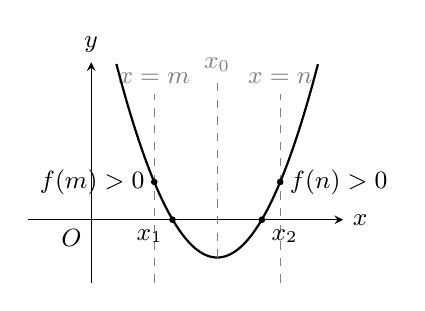
\begin{tikzpicture}[scale=0.8, >=stealth]
  \draw[->] (-1,0) -- (4,0) node[right] {\small $x$};
  \draw[->] (0,-1) -- (0,2.5) node[above] {\small $y$};
  \draw[dashed, gray] (1,-1) -- (1,2) node[above] {\small $x=m$};
  \draw[dashed, gray] (3,-1) -- (3,2) node[above] {\small $x=n$};
  \draw[thick, domain=0.4:3.6, samples=100] plot (\x, {1.2*(\x-2)*(\x-2) - 0.6});
  \fill (1.29,0) circle (1.5pt) node[below left] {\small $x_1$};
  \fill (2.71,0) circle (1.5pt) node[below right] {\small $x_2$};
  \fill (1,0.6) circle (1.5pt) node[left] {\small $f(m)>0$};
  \fill (3,0.6) circle (1.5pt) node[right] {\small $f(n)>0$};
  \draw[dashed, gray] (2,-0.6) -- (2,2.2) node[above] {\small $x_0$};
  \node[below left] at (0,0) {\small $O$};
\end{tikzpicture}\par}\addvspace{0.3em}

几何直观表现为：抛物线被“兜在”区间 $(m, n)$ 内部，顶点下沉且两侧边界向上扬起。
此时的约束条件组为：
\[
\begin{cases}
  \Delta \ge 0 & (\text{确保方程有实根，包含两根相等的情形}) \\
  m < -\dfrac{b}{2a} < n & (\text{控制对称轴在区间内，防止抛物线跑偏}) \\
  f(m) > 0 & (\text{左边界端点值在 } x \text{ 轴上方}) \\
  f(n) > 0 & (\text{右边界端点值在 } x \text{ 轴上方})
\end{cases}
\]

\subsection{2. 在区间 $(m, n)$ 内恰有一根}
此情形较为复杂，需拆分为三种几何位置模型进行分类约束：

\subsubsection{情况 A：两根分居区间边界的两侧（一内一外，不含端点）}
\par\addvspace{0.3em}{\centering
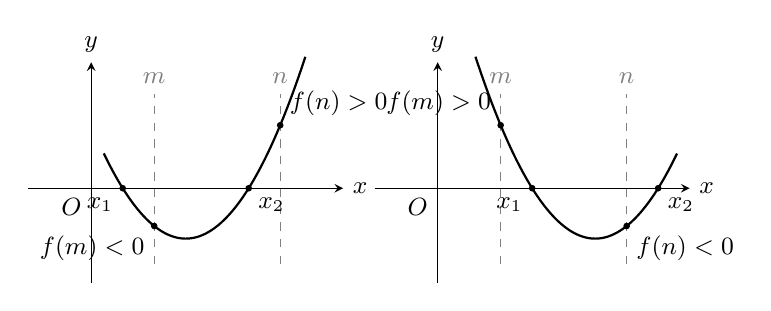
\begin{tikzpicture}[scale=0.8, >=stealth]
  % 左图：左外右内
  \begin{scope}[shift={(0,0)}]
    \draw[->] (-1,0) -- (4,0) node[right] {\small $x$};
    \draw[->] (0,-1.5) -- (0,2) node[above] {\small $y$};
    \draw[dashed, gray] (1,-1.2) -- (1,1.5) node[above] {\small $m$};
    \draw[dashed, gray] (3,-1.2) -- (3,1.5) node[above] {\small $n$};
    \draw[thick, domain=0.2:3.4, samples=100] plot (\x, {0.8*(\x-1.5)*(\x-1.5) - 0.8});
    \fill (0.5,0) circle (1.5pt) node[below left] {\small $x_1$};
    \fill (2.5,0) circle (1.5pt) node[below right] {\small $x_2$};
    \fill (1,-0.6) circle (1.5pt) node[below left] {\small $f(m)<0$};
    \fill (3,1.0) circle (1.5pt) node[above right] {\small $f(n)>0$};
    \node[below left] at (0,0) {\small $O$};
  \end{scope}
  
  % 右图：左内右外
  \begin{scope}[shift={(5.5,0)}]
    \draw[->] (-1,0) -- (4,0) node[right] {\small $x$};
    \draw[->] (0,-1.5) -- (0,2) node[above] {\small $y$};
    \draw[dashed, gray] (1,-1.2) -- (1,1.5) node[above] {\small $m$};
    \draw[dashed, gray] (3,-1.2) -- (3,1.5) node[above] {\small $n$};
    \draw[thick, domain=0.6:3.8, samples=100] plot (\x, {0.8*(\x-2.5)*(\x-2.5) - 0.8});
    \fill (1.5,0) circle (1.5pt) node[below left] {\small $x_1$};
    \fill (3.5,0) circle (1.5pt) node[below right] {\small $x_2$};
    \fill (1,1.0) circle (1.5pt) node[above left] {\small $f(m)>0$};
    \fill (3,-0.6) circle (1.5pt) node[below right] {\small $f(n)<0$};
    \node[below left] at (0,0) {\small $O$};
  \end{scope}
\end{tikzpicture}\par}\addvspace{0.3em}

几何直观表现为：抛物线在区间端点 $m$ 和 $n$ 之间穿过 $x$ 轴一次，因此端点值必然一正一负。
此时的约束条件极其精炼，仅需：
\[
f(m) \cdot f(n) < 0
\]
\begin{graynote}
注：由于端点值异号，抛物线必然在区间内与 $x$ 轴相交，且两根中必有一根在 $(m,n)$ 内、另一根在 $(m,n)$ 外。此时无需再列 $\Delta > 0$ 和对称轴条件。
\end{graynote}

\subsubsection{情况 B：恰有一个重根在区间 $(m, n)$ 内}
\par\addvspace{0.3em}{\centering
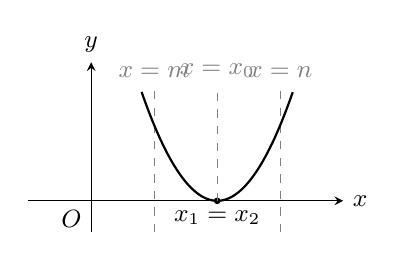
\begin{tikzpicture}[scale=0.8, >=stealth]
  \draw[->] (-1,0) -- (4,0) node[right] {\small $x$};
  \draw[->] (0,-0.5) -- (0,2.2) node[above] {\small $y$};
  \draw[dashed, gray] (1,-0.5) -- (1,1.8) node[above] {\small $x=m$};
  \draw[dashed, gray] (3,-0.5) -- (3,1.8) node[above] {\small $x=n$};
  \draw[thick, domain=0.8:3.2, samples=100] plot (\x, {1.2*(\x-2)*(\x-2)});
  \fill (2,0) circle (1.5pt) node[below] {\small $x_1=x_2$};
  \draw[dashed, gray] (2,0) -- (2,1.8) node[above] {\small $x=x_0$};
  \node[below left] at (0,0) {\small $O$};
\end{tikzpicture}\par}\addvspace{0.3em}

几何直观表现为：抛物线顶点刚好触碰在区间内的 $x$ 轴上。
此时的约束条件组为：
\[
\begin{cases}
  \Delta = 0 & (\text{确保只有一个重根}) \\
  m < -\dfrac{b}{2a} < n & (\text{确保重根在区间内})
\end{cases}
\]

\subsubsection{情况 C：一根在区间 $(m, n)$ 内，另一根刚好在端点上}
\par\addvspace{0.3em}{\centering
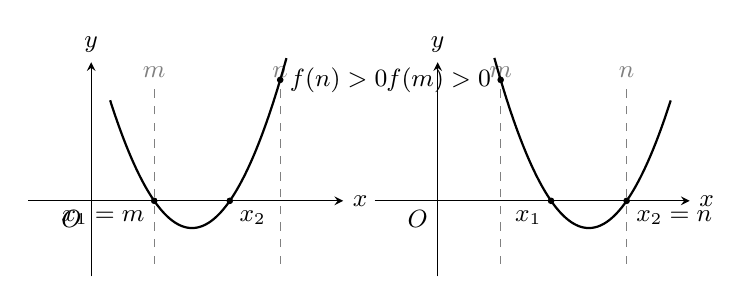
\begin{tikzpicture}[scale=0.8, >=stealth]
  % 左图：左端点为根，另一根在区间内
  \begin{scope}[shift={(0,0)}]
    \draw[->] (-1,0) -- (4,0) node[right] {\small $x$};
    \draw[->] (0,-1.2) -- (0,2.2) node[above] {\small $y$};
    \draw[dashed, gray] (1,-1.0) -- (1,1.8) node[above] {\small $m$};
    \draw[dashed, gray] (3,-1.0) -- (3,1.8) node[above] {\small $n$};
    \draw[thick, domain=0.3:3.1, samples=100] plot (\x, {1.2*(\x-1)*(\x-2.2)});
    \fill (1,0) circle (1.5pt) node[below left] {\small $x_1=m$};
    \fill (2.2,0) circle (1.5pt) node[below right] {\small $x_2$};
    \fill (3,1.92) circle (1.5pt) node[right] {\small $f(n)>0$};
    \node[below left] at (0,0) {\small $O$};
  \end{scope}
  
  % 右图：右端点为根，另一根在区间内
  \begin{scope}[shift={(5.5,0)}]
    \draw[->] (-1,0) -- (4,0) node[right] {\small $x$};
    \draw[->] (0,-1.2) -- (0,2.2) node[above] {\small $y$};
    \draw[dashed, gray] (1,-1.0) -- (1,1.8) node[above] {\small $m$};
    \draw[dashed, gray] (3,-1.0) -- (3,1.8) node[above] {\small $n$};
    \draw[thick, domain=0.9:3.7, samples=100] plot (\x, {1.2*(\x-1.8)*(\x-3)});
    \fill (1.8,0) circle (1.5pt) node[below left] {\small $x_1$};
    \fill (3,0) circle (1.5pt) node[below right] {\small $x_2=n$};
    \fill (1,1.92) circle (1.5pt) node[left] {\small $f(m)>0$};
    \node[below left] at (0,0) {\small $O$};
  \end{scope}
\end{tikzpicture}\par}\addvspace{0.3em}

几何直观表现为：抛物线刚好穿过其中一个端点，而对称轴的位置决定了另一根是否在区间内部。
我们采用\textbf{“先定点、后定范围”}的策略：
\begin{itemize}
  \item \textbf{若左端点 $m$ 是根}：即满足 $f(m)=0$。此时另一根为 $x_2 = -\dfrac{b}{a} - m$。
        要使 $x_2 \in (m, n)$，需满足：
        \[
        m < -\dfrac{b}{a} - m < n \Longleftrightarrow m < -\dfrac{b}{2a} < \dfrac{m+n}{2}
        \]
        \begin{graynote}
        注：由于开口向上，$f(m)=0$ 时，只要对称轴在 $m$ 和中点 $\frac{m+n}{2}$ 之间，即可保证另一根在 $(m,n)$ 内。此时必然有 $f(n)>0$。
        \end{graynote}
  \item \textbf{若右端点 $n$ 是根}：即满足 $f(n)=0$。此时另一根为 $x_1 = -\dfrac{b}{a} - n$。
        要使 $x_1 \in (m, n)$，需满足：
        \[
        m < -\dfrac{b}{a} - n < n \Longleftrightarrow \dfrac{m+n}{2} < -\dfrac{b}{2a} < n
        \]
        \begin{graynote}
        注：同理，只要对称轴在区间中点和右端点 $n$ 之间，即可保证另一根在 $(m,n)$ 内。此时必然有 $f(m)>0$。
        \end{graynote}
\end{itemize}

\subsection{3. 在区间 $(m, n)$ 内没有根}
方程在区间 $(m, n)$ 内没有根，即对应的图象在该区间内与 $x$ 轴无交点。根据抛物线的下沉程度，可分为以下三种模型讨论：

\subsubsection{情况 A：方程根本无实数根}
\par\addvspace{0.3em}{\centering
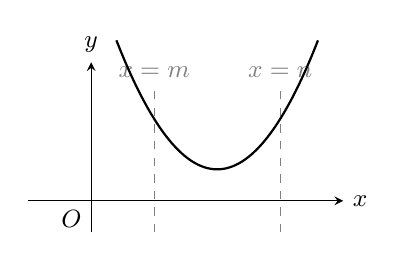
\begin{tikzpicture}[scale=0.8, >=stealth]
  \draw[->] (-1,0) -- (4,0) node[right] {\small $x$};
  \draw[->] (0,-0.5) -- (0,2.2) node[above] {\small $y$};
  \draw[dashed, gray] (1,-0.5) -- (1,1.8) node[above] {\small $x=m$};
  \draw[dashed, gray] (3,-0.5) -- (3,1.8) node[above] {\small $x=n$};
  \draw[thick, domain=0.4:3.6, samples=100] plot (\x, {0.8*(\x-2)*(\x-2) + 0.5});
  \node[below left] at (0,0) {\small $O$};
\end{tikzpicture}\par}\addvspace{0.3em}

几何直观表现为：抛物线悬空，完全在 $x$ 轴上方。
此时的约束条件极其简单：
\[
\Delta < 0
\]

\subsubsection{情况 B：方程有实根，但两根均在区间同侧}
\par\addvspace{0.3em}{\centering
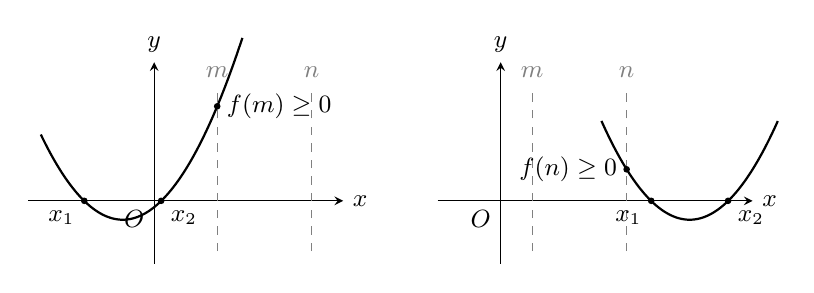
\begin{tikzpicture}[scale=0.8, >=stealth]
  % 左图：两根都在 m 左侧
  \begin{scope}[shift={(0,0)}]
    \draw[->] (-2,0) -- (3,0) node[right] {\small $x$};
    \draw[->] (0,-1.0) -- (0,2.2) node[above] {\small $y$};
    \draw[dashed, gray] (1,-0.8) -- (1,1.8) node[above] {\small $m$};
    \draw[dashed, gray] (2.5,-0.8) -- (2.5,1.8) node[above] {\small $n$};
    \draw[thick, domain=-1.8:1.4, samples=100] plot (\x, {0.8*(\x+0.5)*(\x+0.5) - 0.3});
    \fill (-1.11,0) circle (1.5pt) node[below left] {\small $x_1$};
    \fill (0.11,0) circle (1.5pt) node[below right] {\small $x_2$};
    \fill (1,1.5) circle (1.5pt) node[right] {\small $f(m) \ge 0$};
    \node[below left] at (0,0) {\small $O$};
  \end{scope}
  
  % 右图：两根都在 n 右侧
  \begin{scope}[shift={(5.5,0)}]
    \draw[->] (-1,0) -- (4,0) node[right] {\small $x$};
    \draw[->] (0,-1.0) -- (0,2.2) node[above] {\small $y$};
    \draw[dashed, gray] (0.5,-0.8) -- (0.5,1.8) node[above] {\small $m$};
    \draw[dashed, gray] (2,-0.8) -- (2,1.8) node[above] {\small $n$};
    \draw[thick, domain=1.6:4.4, samples=100] plot (\x, {0.8*(\x-3)*(\x-3) - 0.3});
    \fill (2.39,0) circle (1.5pt) node[below left] {\small $x_1$};
    \fill (3.61,0) circle (1.5pt) node[below right] {\small $x_2$};
    \fill (2,0.5) circle (1.5pt) node[left] {\small $f(n) \ge 0$};
    \node[below left] at (0,0) {\small $O$};
  \end{scope}
\end{tikzpicture}\par}\addvspace{0.3em}

几何直观表现为：抛物线与 $x$ 轴相交，但交点被整体推到了区间的左侧或右侧之外。
\begin{itemize}
  \item \textbf{两根都在 $m$ 左侧（含端点 $m$）}：
        \[
        \begin{cases}
          \Delta \ge 0 \\
          -\dfrac{b}{2a} \le m \\
          f(m) \ge 0
        \end{cases}
        \]
  \item \textbf{两根都在 $n$ 右侧（含端点 $n$）}：
        \[
        \begin{cases}
          \Delta \ge 0 \\
          -\dfrac{b}{2a} \ge n \\
          f(n) \ge 0
        \end{cases}
        \]
\end{itemize}

\subsubsection{情况 C：方程有实根，但区间被夹在两根之间}
\par\addvspace{0.3em}{\centering
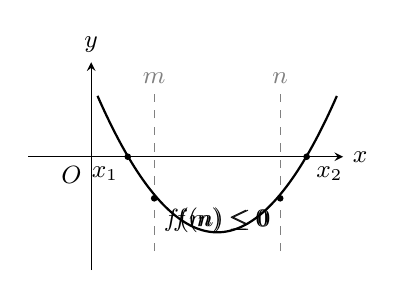
\begin{tikzpicture}[scale=0.8, >=stealth]
  \draw[->] (-1,0) -- (4,0) node[right] {\small $x$};
  \draw[->] (0,-1.8) -- (0,1.5) node[above] {\small $y$};
  \draw[dashed, gray] (1,-1.5) -- (1,1.0) node[above] {\small $m$};
  \draw[dashed, gray] (3,-1.5) -- (3,1.0) node[above] {\small $n$};
  \draw[thick, domain=0.1:3.9, samples=100] plot (\x, {0.6*(\x-2)*(\x-2) - 1.2});
  \fill (0.58,0) circle (1.5pt) node[below left] {\small $x_1$};
  \fill (3.42,0) circle (1.5pt) node[below right] {\small $x_2$};
  \fill (1,-0.66) circle (1.5pt) node[below right] {\small $f(m) \le 0$};
  \fill (3,-0.66) circle (1.5pt) node[below left] {\small $f(n) \le 0$};
  \node[below left] at (0,0) {\small $O$};
\end{tikzpicture}\par}\addvspace{0.3em}

几何直观表现为：抛物线“深陷”在 $x$ 轴下方，整个区间都在其凹陷的腹部内，故两端点处对应函数值均在 $x$ 轴下方或刚好在 $x$ 轴上。
此时约束条件为：
\[
\begin{cases}
  f(m) \le 0 \\
  f(n) \le 0
\end{cases}
\]
\begin{graynote}
注：当且仅当 $f(m)=0$ 且 $f(n)=0$ 时，两根刚好在区间边界上，此时区间内无根。
\end{graynote}

\subsection{例 8.1：两根都大于 $k$}
\begin{exbox}{例题}
已知关于 $x$ 的方程 $x^2 - 2(a-1)x + 4 = 0$ 的两根都大于 1，求实数 $a$ 的取值范围。
\end{exbox}

\begin{paracol}{2}
\teachblock{标准解答与讲解主线}{
  设 $f(x) = x^2 - 2(a-1)x + 4$。
  两根都在 1 的右侧，即 $x_1 \ge 1, x_2 \ge 1$（方程可能有两个相等实根）。
  \begin{center}
  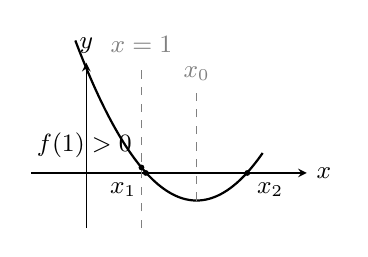
\begin{tikzpicture}[scale=0.7, >=stealth]
    \draw[->] (-1,0) -- (4,0) node[right] {\small $x$};
    \draw[->] (0,-1) -- (0,2) node[above] {\small $y$};
    \draw[dashed, gray] (1,-1) -- (1,2) node[above] {\small $x=1$};
    \draw[thick, domain=-0.2:3.2, samples=100] plot (\x, {0.6*(\x-2)*(\x-2) - 0.5});
    \fill (1.08,0) circle (1.5pt) node[below left] {\small $x_1$};
    \fill (2.92,0) circle (1.5pt) node[below right] {\small $x_2$};
    \fill (1,0.1) circle (1.5pt) node[above left] {\small $f(1)>0$};
    \draw[dashed, gray] (2,-0.5) -- (2,1.5) node[above] {\small $x_0$};
  \end{tikzpicture}
  \end{center}
  列出限制条件组：
  \[
  \begin{cases}
    \Delta = 4(a-1)^2 - 16 \ge 0 \\
    x_0 = a-1 > 1 \\
    f(1) = 1 - 2(a-1) + 4 > 0
  \end{cases}
  \]
  分别求解：
  (1) $(a-1)^2 \ge 4 \implies a-1 \ge 2 \text{ 或 } a-1 \le -2 \implies a \ge 3 \text{ 或 } a \le -1$。
  (2) $a-1 > 1 \implies a > 2$。
  (3) $7-2a > 0 \implies a < \dfrac{7}{2}$。
  
  取交集，最终范围为：
  \[
  \boxed{3 \le a < \frac{7}{2}}
  \]
}
\switchcolumn
\teachblock{易错分析与教学提示}{
  \textbf{学生常见误区：}\\
  学生容易漏掉判别式 $\Delta \ge 0$（认为有了 $f(1)>0$ 且轴在右边就必然有根）或漏掉对称轴。
  
  \textbf{启发与提问口径：}\\
  \begin{itemize}
    \item “如果没有判别式，抛物线可能整体浮在 $x$ 轴上方，此时 $f(1)>0$ 且对称轴也在右边，但方程根本没有根。所以判别式是根存在的基本安全锁。”
  \end{itemize}
}
\end{paracol}

\subsection{例 8.2：一根小于 $k$，一根大于 $k$（两根分居 $k$ 两侧）}
\begin{exbox}{例题}
已知关于 $x$ 的方程 $x^2 - 2ax + a + 2 = 0$ 的一根小于 1，另一根大于 1，求实数 $a$ 的取值范围。
\end{exbox}

\begin{paracol}{2}
\teachblock{标准解答与讲解主线}{
  设 $f(x) = x^2 - 2ax + a + 2$。
  两根分居 1 的两侧，由于开口向上。
  \begin{center}
  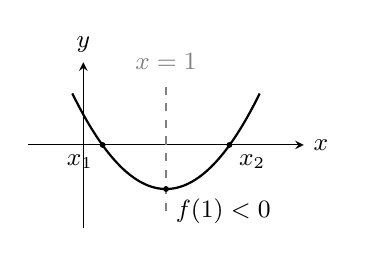
\begin{tikzpicture}[scale=0.7, >=stealth]
    \draw[->] (-1,0) -- (4,0) node[right] {\small $x$};
    \draw[->] (0,-1.5) -- (0,1.5) node[above] {\small $y$};
    \draw[dashed, gray] (1.5,-1.2) -- (1.5,1.2) node[above] {\small $x=1$};
    \draw[thick, domain=-0.2:3.2, samples=100] plot (\x, {0.6*(\x-1.5)*(\x-1.5) - 0.8});
    \fill (0.35,0) circle (1.5pt) node[below left] {\small $x_1$};
    \fill (2.65,0) circle (1.5pt) node[below right] {\small $x_2$};
    \fill (1.5,-0.8) circle (1.5pt) node[below right] {\small $f(1)<0$};
  \end{tikzpicture}
  \end{center}
  我们只需要保证边界点 1 处的函数值小于 0 即可：
  \[
  f(1) < 0 \implies 1 - 2a + a + 2 < 0 \implies 3 - a < 0
  \]
  解得：
  \[
  \boxed{a > 3}
  \]
  （注意：此处不需要列 $\Delta > 0$ 和对称轴讨论，因为 $f(1) < 0$ 已经隐含了抛物线必然与 $x$ 轴相交两次，且 1 在两根之间）。
}
\switchcolumn
\teachblock{易错分析与教学提示}{
  \textbf{学生常见误区：}\\
  学生往往会去做无用功，计算复杂的 $\Delta > 0$ 和对称轴，耽误考试时间。
  
  \textbf{启发与提问口径：}\\
  \begin{itemize}
    \item “抛物线开口向上，如果在 $x=1$ 时它已经掉到 $x$ 轴下方了，那它往左右两边无限延伸的时候是不是必然会穿过 $x$ 轴上去？那就绝对会有两个根，不需要再算判别式了。”
  \end{itemize}
}
\end{paracol}

\newpage

\subsection{例 8.3：恰有一根在区间 $(a,b)$ 内}
\begin{exbox}{例题}
已知方程 $x^2 - 2ax + a + 2 = 0$ 恰有一根在区间 $(0,2)$ 内，求实数 $a$ 的取值范围。
\end{exbox}

\begin{paracol}{2}
\teachblock{标准解答与讲解主线}{
  设 $f(x) = x^2 - 2ax + a + 2$。
  
  \textbf{情况一：一个根在区间内部，另一个根在区间外}\\
  由于开口向上，说明图像在 0 和 2 处一正一负（穿过 $x$ 轴）。
  \begin{center}
  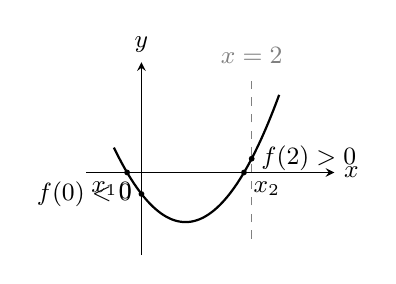
\begin{tikzpicture}[scale=0.7, >=stealth]
    \draw[->] (-1,0) -- (3.5,0) node[right] {\small $x$};
    \draw[->] (0,-1.5) -- (0,2) node[above] {\small $y$};
    \draw[dashed, gray] (2,-1.2) -- (2,1.8) node[above] {\small $x=2$};
    \draw[thick, domain=-0.5:2.5, samples=100] plot (\x, {0.8*(\x-0.8)*(\x-0.8) - 0.9});
    \fill (-0.26,0) circle (1.5pt) node[below left] {\small $x_1$};
    \fill (1.86,0) circle (1.5pt) node[below right] {\small $x_2$};
    \fill (0, -0.39) circle (1.5pt) node[left] {\small $f(0) < 0$};
    \fill (2, 0.25) circle (1.5pt) node[right] {\small $f(2) > 0$};
    \node[below left] at (0,0) {\small $0$};
  \end{tikzpicture}
  \end{center}
  只需列条件：
  \[
  f(0)f(2) < 0 \implies (a+2)(6-3a) < 0 \implies 3(a+2)(a-2) > 0
  \]
  解得：$a > 2$ 或 $a < -2$。
  
  \textbf{情况二：临界端点根讨论}
  \begin{itemize}
    \item 若 $f(0) = 0 \implies a = -2$。此时方程为 $x^2+4x = 0$，根为 $0$ 和 $-4$。区间 $(0,2)$ 内无根。舍去。
    \item 若 $f(2) = 0 \implies a = 2$。此时方程为 $x^2-4x+4 = 0$，根为 $2$（重根）。区间 $(0,2)$ 内无根。舍去。
  \end{itemize}
  
  综上所述，实数 $a$ 的取值范围是 $\boxed{a > 2 \text{ 或 } a < -2}$。
}
\switchcolumn
\teachblock{易错分析与教学提示}{
  \textbf{学生常见误区：}\\
  学生做题时经常忽略端点值等于 0 的临界情况。
  
  \textbf{启发与提问口径：}\\
  \begin{itemize}
    \item “如果有某一个根刚好落在边界 0 或 2 上，它就不在‘开区间’ $(0,2)$ 内了。所以边界端点必须拿出来单独带回原式检验。”
  \end{itemize}
}
\end{paracol}

\subsection{例 8.4：两根都在区间 $(a,b)$ 内}
\begin{exbox}{例题}
已知关于 $x$ 的方程 $x^2 - 2ax + 2 - a = 0$ 的两个根都在区间 $(0,2)$ 内，求实数 $a$ 的取值范围。
\end{exbox}

\begin{paracol}{2}
\teachblock{标准解答与讲解主线}{
  设 $f(x) = x^2 - 2ax + 2 - a$。
  两根都在区间内，我们需要用“四重锁”把抛物线框死在区间内：
  \begin{center}
  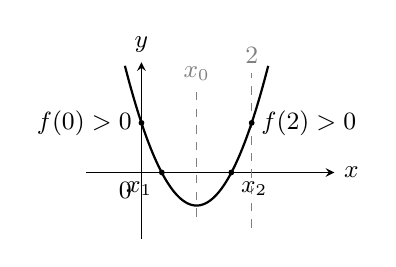
\begin{tikzpicture}[scale=0.7, >=stealth]
    \draw[->] (-1,0) -- (3.5,0) node[right] {\small $x$};
    \draw[->] (0,-1.2) -- (0,2) node[above] {\small $y$};
    \draw[dashed, gray] (2,-1) -- (2,1.8) node[above] {\small $2$};
    \draw[thick, domain=-0.3:2.3, samples=100] plot (\x, {1.5*(\x-1)*(\x-1) - 0.6});
    \draw[dashed, gray] (1,-0.8) -- (1,1.5) node[above] {\small $x_0$};
    \fill (0.37,0) circle (1.5pt) node[below left] {\small $x_1$};
    \fill (1.63,0) circle (1.5pt) node[below right] {\small $x_2$};
    \fill (0, 0.9) circle (1.5pt) node[left] {\small $f(0) > 0$};
    \fill (2, 0.9) circle (1.5pt) node[right] {\small $f(2) > 0$};
    \node[below left] at (0,0) {\small $0$};
  \end{tikzpicture}
  \end{center}
  列出条件组：
  \[
  \begin{cases}
    \Delta = 4a^2 - 4(2-a) \ge 0 \\
    0 < x_0 = a < 2 \\
    f(0) = 2-a > 0 \\
    f(2) = 4-4a+2-a = 6-5a > 0
  \end{cases}
  \]
  求解各不等式：
  (1) $a^2+a-2 \ge 0 \implies (a+2)(a-1) \ge 0 \implies a \ge 1 \text{ 或 } a \le -2$。
  (2) $0 < a < 2$。
  (3) $a < 2$。
  (4) $a < \dfrac{6}{5}$。
  
  取交集，最终范围为：
  \[
  \boxed{\left[1, \frac{6}{5}\right)}
  \]
}
\switchcolumn
\teachblock{易错分析与教学提示}{
  \textbf{学生常见误区：}\\
  “四重锁”少写了其中一个（例如对称轴或某端点），导致范围被扩大。
  
  \textbf{启发与提问口径：}\\
  \begin{itemize}
    \item “我们为什么要列这么多条件？为了把抛物线逼到 $(0,2)$ 里面去。如果只写 $f(0)>0, f(2)>0$，对称轴可能在外面，或者抛物线飞起来了没有根。必须由 $\Delta$ 保证有根，对称轴控制位置，两个端点向上托住，合力锁死。”
  \end{itemize}
}
\end{paracol}

\newpage

\subsection{例 8.5：一根在区间 $(a,b)$ 内，另一根在区间 $(c,d)$ 内}
\begin{exbox}{例题}
已知关于 $x$ 的方程 $x^2 - (2a-1)x + a^2 - a = 0$ 的一根在区间 $(0,1)$ 内，另一根在区间 $(1,2)$ 内，求实数 $a$ 的取值范围。
\end{exbox}

\begin{paracol}{2}
\teachblock{标准解答与讲解主线}{
  设 $f(x) = x^2 - (2a-1)x + a^2 - a$。
  
  \textbf{解法一：因式分解（捷径视角）}\\
  观察方程左侧，常数项可因式分解：$a^2-a = a(a-1)$。
  同时，一次项系数 $-(2a-1) = -[a + (a-1)]$。
  故原方程可以直接十字相乘分解：
  \[
  (x-a)[x-(a-1)] = 0
  \]
  方程的两根分别为：$x_1 = a-1$ 和 $x_2 = a$。
  因为 $a-1 < a$，所以较小根是 $a-1$，较大根是 $a$。
  依题意，一根在 $(0,1)$ 内，另一根在 $(1,2)$ 内，必须满足：
  \[
  \begin{cases}
    0 < a-1 < 1 \\
    1 < a < 2
  \end{cases}
  \implies
  \begin{cases}
    1 < a < 2 \\
    1 < a < 2
  \end{cases}
  \]
  解得：$\boxed{1 < a < 2}$。
  
  \textbf{解法二：常规根分布条件}\\
  两根被 1 分开，且分别被 0 和 2 包围在里面。
  根据图像的连通性，从左到右四个点 $0,1,2$ 处的函数值必须满足“正、负、正”的关系：
  \begin{center}
  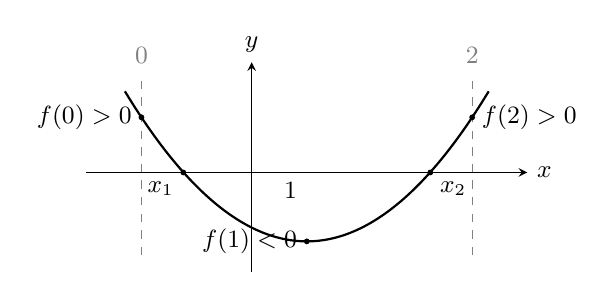
\begin{tikzpicture}[scale=0.7, >=stealth]
    \draw[->] (-3,0) -- (5,0) node[right] {\small $x$};
    \draw[->] (0,-1.8) -- (0,2) node[above] {\small $y$};
    \draw[dashed, gray] (-2,-1.5) -- (-2,1.8) node[above] {\small $0$};
    \draw[dashed, gray] (4,-1.5) -- (4,1.8) node[above] {\small $2$};
    \draw[thick, domain=-2.3:4.3, samples=100] plot (\x, {0.25*(\x-1)*(\x-1) - 1.25});
    \fill (-1.24,0) circle (1.5pt) node[below left] {\small $x_1$};
    \fill (3.24,0) circle (1.5pt) node[below right] {\small $x_2$};
    \fill (-2, 1.0) circle (1.5pt) node[left] {\small $f(0) > 0$};
    \fill (1, -1.25) circle (1.5pt) node[left] {\small $f(1) < 0$};
    \fill (4, 1.0) circle (1.5pt) node[right] {\small $f(2) > 0$};
    \node[below left] at (1,0) {\small $1$};
  \end{tikzpicture}
  \end{center}
  列出条件组：
  \[
  \begin{cases}
    f(0) = a^2-a > 0 \implies a>1 \text{ 或 } a<0 \\
    f(1) = 1-(2a-1)+a^2-a = a^2-3a+2 < 0 \implies 1<a<2 \\
    f(2) = 4-2(2a-1)+a^2-a = a^2-5a+6 > 0 \implies a>3 \text{ 或 } a<2
  \end{cases}
  \]
  取交集，同样解得：$\boxed{1 < a < 2}$。
}
\switchcolumn
\teachblock{易错分析与教学提示}{
  \textbf{学生常见误区：}\\
  学生往往想不到可以因式分解，直接套用复杂的解法二，这会导致计算量偏大，容易算错。
  
  \textbf{启发与提问口径：}\\
  \begin{itemize}
    \item “在做一元二次方程题的时候，我们脑子里的第一步决策应该是什么？\textbf{先看看能不能因式分解！}如果能直接求出根，这道题的难度就会从根的分布降到一元一次不等式组，能节省大把时间。”
  \end{itemize}
}
\end{paracol}

\newpage

\section{第 9 讲：复杂函数中的恒成立与有解}

无论函数的解析式如何复杂，处理参数范围的核心思想依旧保持一致。我们优先求出辅助函数的值域或最值，再进行不等式翻译。

\subsection{1. 绝对值函数与图线分析}
绝对值不等式往往可以通过分段讨论法，或者绝对值的几何意义（数轴两点间距离）进行化简破局。

\subsection{2. 对数函数与定义域优先法则}
对数问题中，\textbf{定义域真数大于 0 是第一守门条件}。在进行任何对数恒成立转换前，必须优先写出定义域限制。

\subsection{3. 三角函数的值域转换}
利用辅助角公式 $a\sin x + b\cos x = \sqrt{a^2+b^2}\sin(x+\varphi)$，将复杂三角不等式化为简谐振动形式，再利用值域区间进行范围锁定。

\begin{exbox}{例 9.1}
已知不等式 $|x-1| + |x-2| \ge a$ 对任意 $x \in \mathbb R$ 恒成立，求实数 $a$ 的取值范围。
\end{exbox}

\begin{paracol}{2}
\teachblock{标准解答与讲解主线}{
  \textbf{解题思路：}\\
  根据恒成立法则，原不等式等价于：
  \[
  a \le (|x-1| + |x-2|)_{\min}
  \]
  我们只需求出辅助函数 $g(x) = |x-1| + |x-2|$ 的最小值即可。
  
  \textbf{几何解释：}\\
  $|x-1| + |x-2|$ 在数轴上表示自变量 $x$ 到点 $1$ 与点 $2$ 的距离之和。
  根据绝对值的三角不等式：
  \[
  |x-1| + |x-2| \ge |(x-1) - (x-2)| = 1
  \]
  当且仅当 $1 \le x \le 2$ 时，等号成立。
  因此，辅助函数的最小值为 $1$。
  
  所以，实数 $a$ 的取值范围为：
  \[
  \boxed{a \le 1}
  \]
}
\switchcolumn
\teachblock{易错分析与教学提示}{
  \textbf{学生常见误区：}\\
  学生习惯于写成分段函数去掉绝对值，虽然最终也能做出，但是极其浪费时间。
  
  \textbf{启发与提问口径：}\\
  \begin{itemize}
    \item “绝对值的几何意义是距离。两个绝对值相加，就是‘数轴上一个点到 1 和 2 的距离之和’。为了让这个距离和最小，这个点应该在哪？肯定在 1 和 2 之间。此时距离之和就是 1 到 2 的距离，即为 1。”
  \end{itemize}
}
\end{paracol}

\begin{exbox}{例 9.2}
已知对任意 $x \in [1,2]$，不等式 $\dfrac{x-a}{x+1} \ge 0$ 恒成立，求实数 $a$ 的取值范围。
\end{exbox}

\begin{paracol}{2}
\teachblock{标准解答与讲解主线}{
  \textbf{解题步骤：}\\
  因为 $x \in [1,2]$，所以分母 $x+1 \ge 2 > 0$ 恒成立。
  既然分母恒为正，要使分式大于等于 0，只需分子大于等于 0 即可：
  \[
  x-a \ge 0 \Longleftrightarrow a \le x
  \]
  这要求对任意 $x \in [1,2]$ 恒成立，故等价于：
  \[
  a \le x_{\min} \quad (x \in [1,2])
  \]
  显然，在区间 $[1,2]$ 上，自变量 $x$ 的最小值为 $1$。
  
  所以，实数 $a$ 的取值范围是：
  \[
  \boxed{a \le 1}
  \]
}
\switchcolumn
\teachblock{易错分析与教学提示}{
  \textbf{学生常见误区：}\\
  学生往往容易把分式不等式想得太复杂，试图去求导或做除法分离参数，做了无用功。
  
  \textbf{启发与提问口径：}\\
  \begin{itemize}
    \item “一个分式是正数，在分母已经是正数的情况下，分子必须是什么数？必须是正数。所以直接去掉分母，就变成了一次不等式。”
  \end{itemize}
}
\end{paracol}

\begin{exbox}{例 9.3}
已知对任意 $x \in \mathbb R$，不等式 $a\sin x + \cos x + 2 \ge 0$ 恒成立，求实数 $a$ 的取值范围。
\end{exbox}

\begin{paracol}{2}
\teachblock{标准解答与讲解主线}{
  \textbf{解题步骤：}\\
  原不等式等价于：
  \[
  a\sin x + \cos x \ge -2
  \]
  要使上式对一切 $x \in \mathbb R$ 恒成立，根据恒成立的最值法则，只需：
  \[
  (a\sin x + \cos x)_{\min} \ge -2
  \]
  利用辅助角公式变形左侧：
  \[
  a\sin x + \cos x = \sqrt{a^2+1}\sin(x+\varphi)
  \]
  其中 $\tan\varphi = \dfrac{1}{a}$。
  由于 $x \in \mathbb R$，正弦函数的值域为 $[-1,1]$。
  故左边表达式的最小值为 $-\sqrt{a^2+1}$。
  我们只需：
  \[
  -\sqrt{a^2+1} \ge -2 \Longleftrightarrow \sqrt{a^2+1} \le 2
  \]
  两边平方：
  \[
  a^2+1 \le 4 \implies a^2 \le 3 \implies -\sqrt{3} \le a \le \sqrt{3}
  \]
  
  故实数 $a$ 的取值范围是：
  \[
  \boxed{[-\sqrt{3}, \sqrt{3}]}
  \]
}
\switchcolumn
\teachblock{易错分析与教学提示}{
  \textbf{学生常见误区：}\\
  部分学生会对三角函数的辅助角公式遗忘。或者在解不等式 $-\sqrt{a^2+1} \ge -2$ 时，两边直接平方而忽略了负号导致不等号方向写错。
  
  \textbf{启发与提问口径：}\\
  \begin{itemize}
    \item “遇到 $a\sin x + b\cos x$ 这种复合三角形式，第一步永远是利用辅助角公式将其融合成一个单一的 $\sin$ 形式。因为它的值域就是 $[-\sqrt{a^2+b^2}, \sqrt{a^2+b^2}]$，一目了然。”
  \end{itemize}
}
\end{paracol}

\newpage

\section{专题总结与学生自查决策流程}

\subsection{1. 易错防漏检查点（5 大雷区）}
\begin{enumerate}
  \item \textbf{二次项系数含参}：首项含参第一步必须讨论二次项系数是否为 0。
  \item \textbf{判别式等号取舍}：题目是“两个实根”（$\Delta \ge 0$）还是“两个不等实根”（$\Delta > 0$）必须仔细甄别。
  \item \textbf{有解与恒成立搞混}：恒成立卡最值（大于恒成立看最小，小于看最大），有解卡值域（大于有解看最大，小于看最小）。
  \item \textbf{开区间端点遗漏}：开区间最值在端点取得时，检验是否可以取到该极限值，用“代入检验法”最终核实等号。
  \item \textbf{定义域真数漏写}：对数函数先写真数大于 0。
\end{enumerate}

\subsection{2. 解决函数参数题的“大脑扫描决策 6 步流程”}

\begin{center}
\begin{tcolorbox}[colback=white, colframe=black, boxrule=0.5pt, arc=0pt, left=8pt, right=8pt, top=8pt, bottom=8pt]
\textbf{【参数问题解题决策模板】}
\begin{enumerate}[label=第\arabic*步：, leftmargin=3.5em]
  \item \textbf{锁定变量与参数}：区分变量与参数。若参数只在一次项，考虑主参换位。
  \item \textbf{写出定义域范围}：明确 $x$ 的区间是 $\mathbb R$ 还是有限区间，对于对数背景优先写出真数大于 0。
  \item \textbf{翻译不等式逻辑}：判断是“恒成立”（压最值）还是“有解”（求值域）。
  \item \textbf{尝试分离参数}：优先考虑分离参数法。若能分离成 $a \ge g(x)$ 形式，则求 $g(x)$ 的最值。
  \item \textbf{分类或数形结合}：若无法分离参数，根据开口、对称轴与区间相对位置分类讨论，或者画出图形列条件组。
  \item \textbf{独立验证端点边界}：对于分类边界或区间端点，将临界值代回原方程进行核实，最终确定答案等号。
\end{enumerate}
\end{tcolorbox}
\end{center}

\subsection{3. 高中函数与参数问题核心思维工具箱}
在完成本专题的学习后，学生应当在脑海中建立起以下数学思维的反射弧：
\begin{description}
  \item[函数思维] 式子不是死的，它是一个函数，它会随着变量的变化而流动。
  \item[定义域优先思维] 看到根号、分母、对数，先写定义域。这是最基本的习惯。
  \item[图像与数形结合思维] 方程是交点，不等式是上下，绝对值是距离。代数算不动，就换成图像。
  \item[最值思维] 恒成立看最坏情况（卡住最低点），有解看最好机会（翻过最低门槛）。
  \item[分类讨论思维] 分类不是因为麻烦，而是因为对象的性质发生了改变（如二次项系数是否为0，对称轴与区间相对位置的变化）。
  \item[充分必要思维] 别把必要条件当成答案。列完条件后，务必自问：这些条件合起来充分吗？
  \item[边界思维] 等号能不能取？边界情况是否满足原题？最后一步永远记得“代回边界点做最终检验”。
  \item[交并意识] 一条路内取交集，多条路之间取并集。
  \item[结构与代换思维] 抓结构，不要一味展开。善于进行整体代换（如换元 $t = |x|$ 或 $t = x^2-2x$）。
\end{description}

\end{document}
